% Autor: Leonhard Segger, Alexander Neuwirth
% Datum: 2017-10-30
\documentclass[
	% Papierformat
	a4paper,
	% Schriftgröße (beliebige Größen mit „fontsize=Xpt“)
	12pt,
	% Schreibt die Papiergröße korrekt ins Ausgabedokument
	pagesize,
	% Sprache für z.B. Babel
	ngerman
]{scrartcl}

% Achtung: Die Reihenfolge der Pakete kann (leider) wichtig sein!
% Insbesondere sollten (so wie hier) babel, fontenc und inputenc (in dieser
% Reihenfolge) als Erstes und hyperref und cleveref (Reihenfolge auch hier
% beachten) als Letztes geladen werden!

%Malen
\usepackage{tikz}
\usetikzlibrary{calc,patterns,angles,quotes} % loads some tikz extensions\usepackage{tikz}
\usetikzlibrary{babel}

% Silbentrennung etc.; Sprache wird durch Option bei \documentclass festgelegt
\usepackage{babel}
% Verwendung der Zeichentabelle T1 (Sonderzeichen etc.)
\usepackage[T1]{fontenc}
% Legt die Zeichenkodierung der Eingabedatei fest, z.B. UTF-8
\usepackage[utf8]{inputenc}
% Schriftart
\usepackage{lmodern}
% Zusätzliche Sonderzeichen
\usepackage{textcomp}

% Mathepaket (intlimits: Grenzen über/unter Integralzeichen)
\usepackage[intlimits]{amsmath}
% Ermöglicht die Nutzung von \SI{Zahl}{Einheit} u.a.
\usepackage{siunitx}
% Zum flexiblen Einbinden von Grafiken (\includegraphics)
\usepackage{graphicx}
% Abbildungen im Fließtext
\usepackage{wrapfig}
% Abbildungen nebeneinander (subfigure, subtable)
\usepackage{subcaption}
% Funktionen für Anführungszeichen
\usepackage{csquotes}
\MakeOuterQuote{"}
% Zitieren, Bibliografie
\usepackage[sorting=none]{biblatex}


% Zur Darstellung von Webadressen
\usepackage{url}
%chemische Formeln
\usepackage[version=4]{mhchem}
% siunitx: Deutsche Ausgabe, Messfehler getrennt mit ± ausgeben
\usepackage{floatrow}
\floatsetup[table]{capposition=top}
\usepackage{float}
% Verlinkt Textstellen im PDF-Dokument
\usepackage[unicode]{hyperref}
% "Schlaue" Referenzen (nach hyperref laden!)
\usepackage{cleveref}
\sisetup{
	locale=DE,
	separate-uncertainty
}
\bibliography{BA-C-04_EDX_22-10-2018_References}


\begin{document}

	\begin{titlepage}
		\centering
		{\scshape\LARGE Versuchsbericht zu \par}
		\vspace{1cm}
		{\scshape\huge EDX - Energiedispersive Röntgenspektroskopie \par}
		\vspace{2.5cm}
		{\LARGE Gruppe BA-C-04 \par}
		\vspace{0.5cm}

		{\large Alexander Neuwirth (E-Mail: a\_neuw01@wwu.de) \par}
		{\large Leonhard Segger (E-Mail: l\_segg03@uni-muenster.de) \par}
		\vfill

		durchgeführt am 22.10.2018\par
		betreut von\par
		{\large Johann Preuß}

		\vfill

		{\large \today\par}
	\end{titlepage}
	\tableofcontents
	\newpage


	\section{Kurzfassung}
	Die Energiedispersive Röntgenspektroskopie ist ein Verfahren, welches es erlaubt mithilfe des von einer Probe, die mit einem Röntgenstrahl von kontinuierlichem Spektrum beschossen wird, ausgesandten Röntgenfluoreszenzspektrums die Zusammensetzung der Probe zu bestimmen.
	Es sollen mithilfe eines Röntgengeräts und einigen bekannten Proben Röntgenfluoreszenzspektren verschiedener unbekannter Proben aufgezeichnet werden. %sollen kann man denke ich so benutzen...kp, ob Preuß dafür intelligent genut ist.
	Auf Basis dieser Spektren wird die elementare Zusammensetzung der unbekannten Proben untersucht, wobei nicht nur die Art der vorkommenden Elemente, sondern auch ihr Massenanteil an der Gesamtprobe bestimmt wird.
	Hierbei können die Vermutungen, die auf Basis des Aussehens der Proben bestehen, größtenteils bestätigt werden.
	Es werden jedoch auch die Limitierungen des Verfahrens an verschiedenen Beispielen aufgezeigt.
	Zusätzlich kann das Moseleysche Gesetz exemplarisch bestätigt werden und die Abschirmkonstanten von sechs Elementen werden bestimmt.

	%\section{Einführung} %optional


	\section{Methoden}
	Für die Versuchsdurchführung werden ein Röntgengerät, ein Vielkanalanalysator und 21 verschiedene Proben größtenteils unbekannter Natur verwendet.
	Das Röntgengerät, welches mit einer Eisen-Anode arbeitet, und die Proben sind in \cref{fig_aufbau} dargestellt.
	In der Röntgenröhre werden Elektronen beschleunigt.
	Wenn diese auf die Anode treffen, entsteht einerseits Bremsstrahlung, da sie gebremst werden und beschleunigte Ladung elektromagnetische Wellen aussendet. %fine?
	Zum anderen entsteht charakteristische Strahlung dadurch, dass die einfallenden Elektronen Anodenatome ionisieren, indem sie Elektronen niedriger Schalen aus dem Atom herausschlagen.
	Wenn dann Elektronen höherer Schalen in die freigewordene Position herunterfallen, wird charakteristische Strahlung frei.

	Die Röntgenphotonen der charakteristischen Strahlung und Bremsstrahlung können durch eine Blende in die Versuchskammer eintreten, in der sich ein Probenhalter und eine PIN-Diode befinden.

	Das gleiche Prinzip kann durch die Röntgenstrahlung selbst ausgelöst werden.
	Hierbei wird das Atom nicht durch ein Elektron, sondern durch ein Röntgenphoton ionisiert.
	Die hier auftretende charakterische Strahlung wird in diesem Versuch durch die Detektordiode detektiert.

	Die Diode ist mit dem Vielkanalanalysator verbunden.
	In der Diode werden durch die einfallende Strahlung Elektron-Loch-Paare erzeugt.
	Diese werden im elektrischen Feld der angelegten Spannung getrennt und laden einen Rückkopplungskondensator auf, weshalb am Ausgang eines Vorverstärkers eine Spannung in Abhängigkeit von der Anzahl der entstandenen Elektron-Loch-Paare gemessen wird.
	Die verstärkte Spannung wird dann durch einen A/D-Wandler in einen digitalen Wert umgewandelt.
	Hier wird ausgenutzt, dass die Anzahl der in der Detektordiode erzeugten Elektron-Loch-Paare als proportional zur Energie des eingetretenen Röntgenphotons angenommen werden kann.
	Der Vielkanalanalysator generiert hieraus ein Pulshöhenspektrum, indem er die Anzahl der Signale einer bestimmten Spannung summiert, sodass dann Anzahl der Impulse gegen die Impulshöhe aufgetragen werden kann.

	Das Röntgengerät wird mit einer Spannung von \SI{35}{\kilo \electronvolt} betrieben, weshalb dies die erwartete maximal messbare Energie eines Röntgenphotons ist.
	Zusätzlich ist zu beachten, dass der verwendete Röntgenergiedetektor einen Messbereich von \SIrange{2}{58}{keV} hat.

	Zunächst wird der Probenhalter in einen Winkel von \SI{45}{\degree} und der Detektor in einen Winkel von \SI{90}{\degree} zum Röntgenstrahl gebracht.
	Diese Winkel werden mit dem Goniometer eingestellt, obwohl die Verwendung dessen zu einer Stellung führt, die nach Augenmaß nicht exakt den gewünschten Winkeln entspricht, da dies die größere Zählrate zur Folge hatte.

	Um dem verwendeten Messprogramm zu erlauben, den Proportionalitätsfaktor zwischen Pulshöhe und Energie des Röntgenphotons zu bestimmen, wird mit zwei Proben, von denen bekannt ist, aus welchen Elementen sie bestehen, kalibriert.
	Zur Kalibrierung wird Eisen und Molybdän verwendet (Dreipunktkalibrierung).

	Dann werden die Röntgenfluoreszenzspektren aller Proben aufgezeichnet und jeweils Gauß-Fits über die Peaks durchgeführt.
	Es wird jeweils über einen Zeitraum von \SI{10}{\minute} gemessen.
	Die Fitparameter werden verwendet, um Energie, Standardunsicherheit und Höhe des Peaks zu bestimmen.
	Nun können mithilfe dieser Werte und bekannten Übergangsenergien in verschiedenen Elementen die Zusammensetzungen der Proben untersucht bzw. überprüft werden.


	\begin{figure}[H]
		\centering
		\begin{subfigure}[t]{0.5\textwidth}
			\centering
			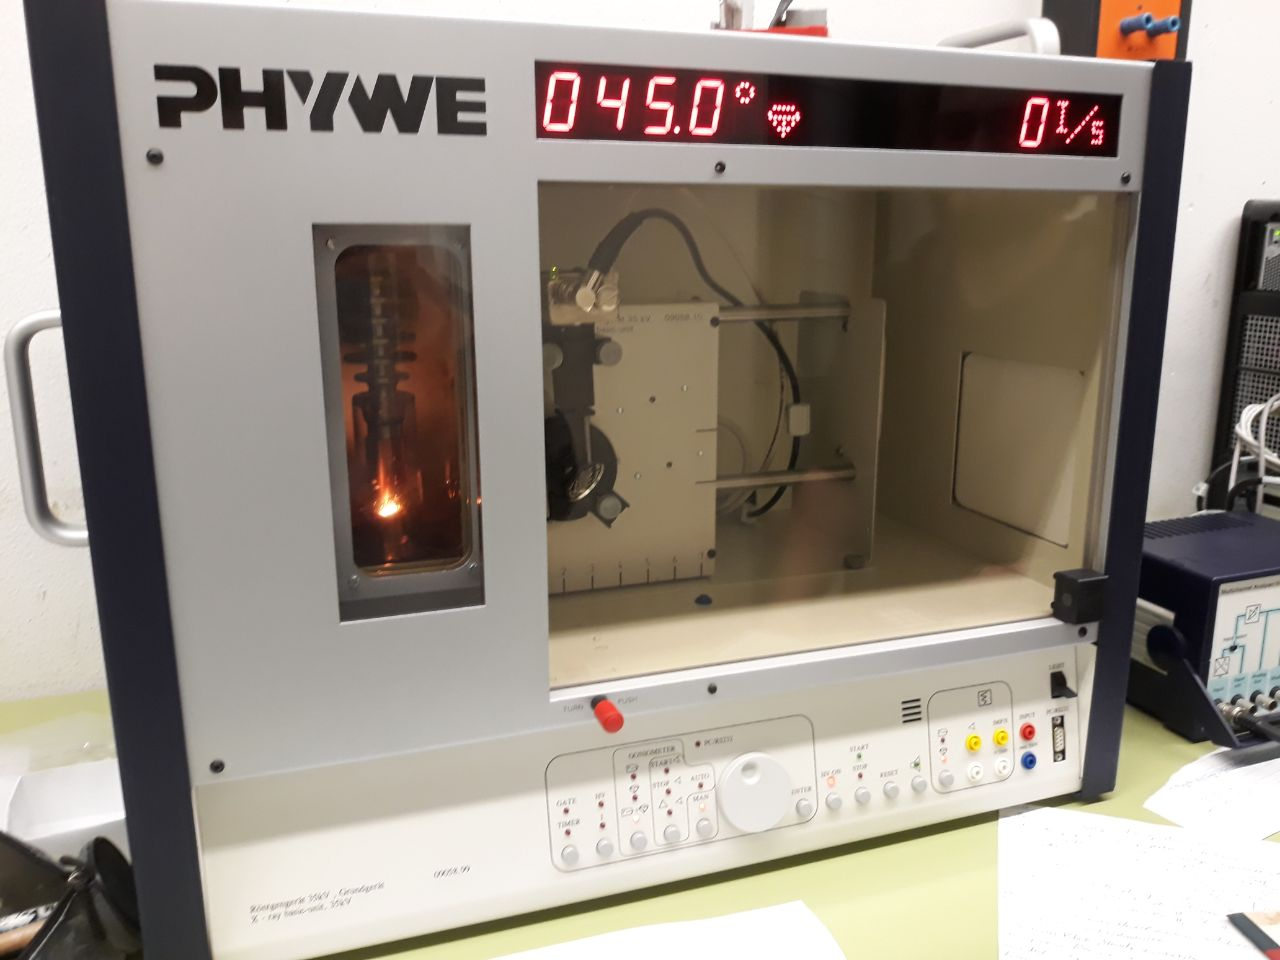
\includegraphics[width=1\textwidth]{images/aufbau}
			\label{fig_aufb_geraet}
			\caption{Röntgengerät}
		\end{subfigure}%
		\begin{subfigure}[t]{0.5\textwidth}
			\centering
			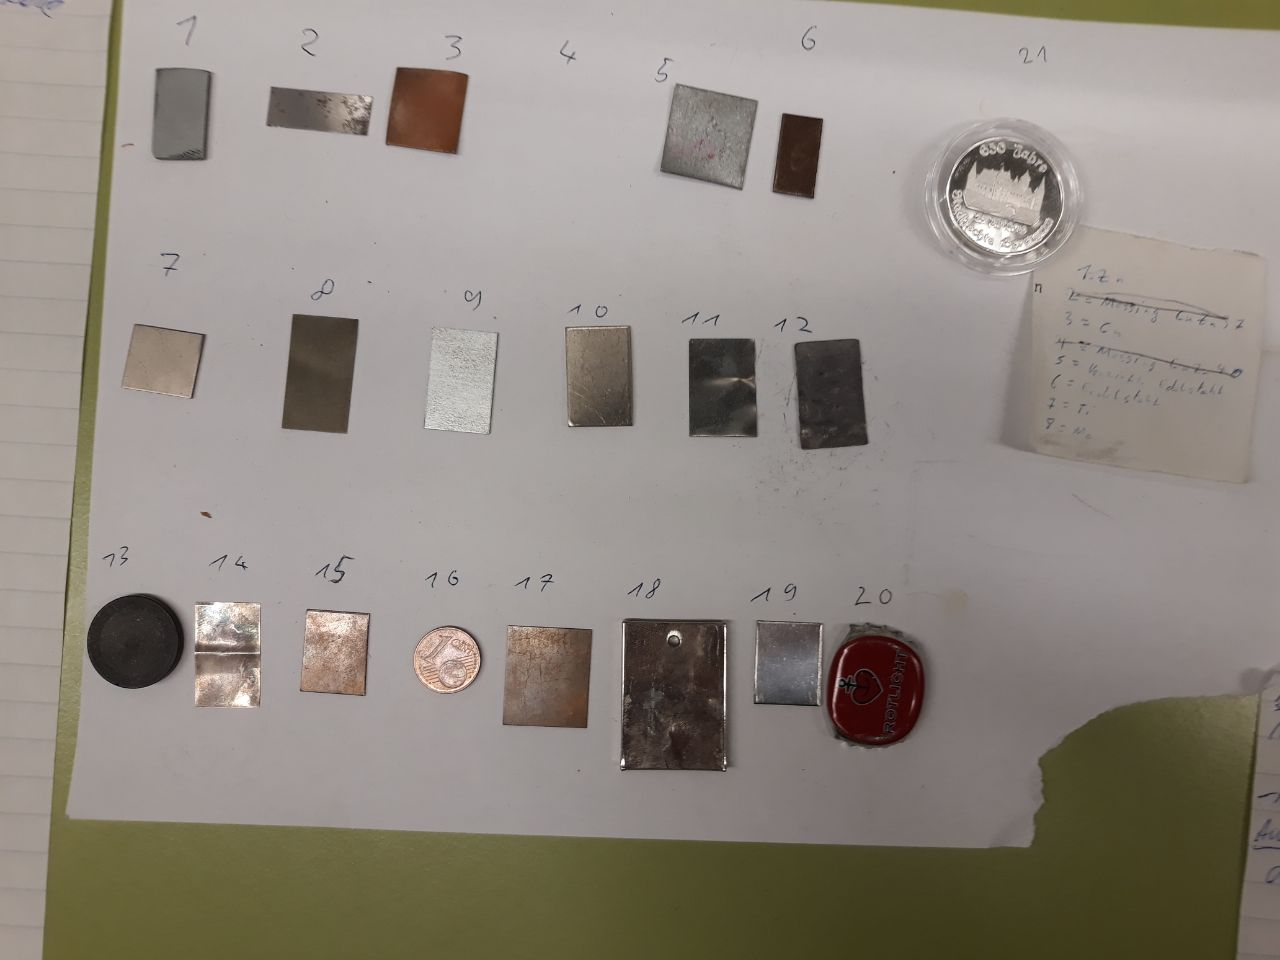
\includegraphics[width=1\textwidth]{images/proben}
			\label{fig_aufb_proben}
			\caption{Proben}
		\end{subfigure}
		\caption{
			\label{fig_aufbau}
			Verwendetes Röntgengerät und Proben. Die Probe mit der Nummer Vier ist nicht im Bild, da sie zum Zeitpunkt der Aufnahme gerade gemessen wurde.}
		\centering

	\end{figure}

	\section{Ergebnisse und Diskussion}


	\subsection{Beobachtung}
	\cref{fig_ag_plot} stellt das Röntgenfluoreszenzspektrum von Probe 21, einer Silbermünze, dar.
	Es ist exemplarisch für die 20 anderen Spektren.
	Alle Spektren haben ein oder zwei dominante und einige weniger ausgeprägte Peaks.
	An den Stellen ohne Peaks wird ein Rauschen von geringer Intensität gemessen.
	Im Anhang befinden sich die gemessenen Spektren, sowie die gefitteten Gauß-Kurven.
	\begin{figure}[H]
		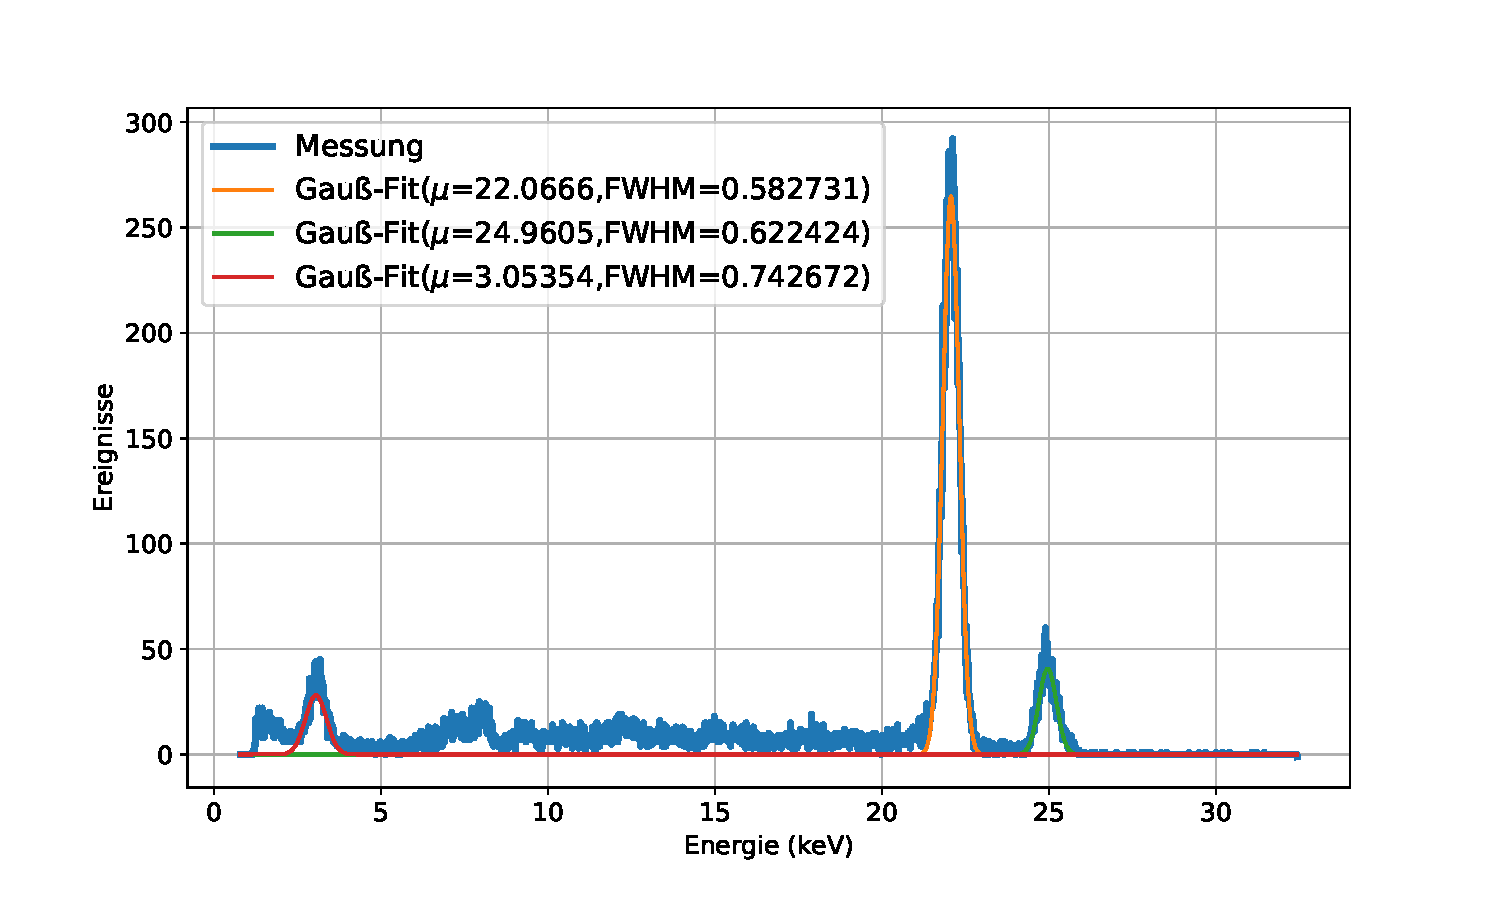
\includegraphics[width=1.0\textwidth]{images/21-Ag}
		\centering
		\caption{Röntgenfluoreszenzspektrum einer Silbermünze. Die Peaks der $\text{L}_\alpha$ (\SI{3,05}{\kilo \electronvolt}), $\text{K}_\alpha$ (\SI{22,07}{\kilo \electronvolt}) und $\text{K}_\beta$ (\SI{25,0}{\kilo \electronvolt}) Linien sind deutlich zu erkennen. Abseits dieser Peaks sind mehrere weitere signifikante Abweichungen von Null zu erkennen, in die aber kein Gauß-Fit gelegt werden kann.}
		\label{fig_ag_plot}
		\centering
	\end{figure}

	\subsection{Datenanalyse}
	\subsubsection{Bestimmung der Abschirmkonstanten}
	Aus den gemessenen Energiespektren wurden die Energien der Peaks mittels eines Gauß-Fits bestimmt.
	Die Standardabweichung ergibt sich dabei aus der FWHM (Full-Width-at-Half-Maximum, Halbwertsbreite):
	\begin{equation}
		\sigma = \frac{\text{FWHM}}{2\sqrt{\ln 2}}
	\end{equation}
	Die Ergebnisse sind in \cref{tb_peaks_known} und \cref{tb_peaks_unknown} aufgeführt.


	\begin{table}[H]
		\centering
		\resizebox{\textwidth}{!}{
		\begin{tabular}{ c | c | c || c | c | c }
			Probe (Angabe)&Energie $E_\text{Mess}$ in \SI{}{keV} & rel. Höhe & Element & char. Übergang &  Energie $E_\text{NIST}$ in \SI{}{keV} \\ \hline \hline

			1 (Zn)
			& \SI{6.38034+-0.139418}{} &\SI{8}{\%}& (Fe) &  K$_\alpha$&\SI{6.3910264(99)}{}\\
			& \SI{8.58804+-0.116621}{} &\SI{79}{\%}&Zn &$\text{K}_\alpha$&  \SI{8.615823(73)}{} \\
			& \SI{9.53296+-0.110738}{} &\SI{13}{\%}&Zn &$\text{K}_\beta$ &  \SI{9.57203(22)}{} \\
			\hline

			2 (Fe)
			& \SI{3.44288+-0.167796}{} &\SI{1}{\%}&(Sn) &  L$_\alpha$& \SI{3 .437356(56) }{} \\
			& \SI{6.39075+-0.117693}{} &\SI{86}{\%}&Fe& $\text{K}_\alpha$ &  \SI{6.3910264(99)}{} \\
			& \SI{7.08998+-0.0953308}{} &\SI{13}{\%}&Fe& $\text{K}_\beta$&  \SI{7.058175(99)}{} \\
			 \hline

			3 (Cu)
			& \SI{8.00053+-0.116792}{} &\SI{86}{\%}&Cu& $\text{K}_\alpha$ &  \SI{8.0278416(26)}{} \\
			& \SI{8.87574+-0.104736}{} &\SI{14}{\%}&Cu& $\text{K}_\beta$ &  \SI{8.905413(38) }{}  \\ \hline

			7 (Ti)
			& \SI{1.39218+-0.0475828}{} &\SI{2}{\%}&-& -&  -\SI{}{} \\
			& \SI{2.54705+-0.281081}{} &\SI{3}{\%}&(Mo)& L$_\alpha$&  \SI{2. 47307(22)    }{} \\
			&&&(Zr)&L$_\beta$& \SI{ 2. 50287(22) }{} \\
			& \SI{4.54007+-0.135133}{} &\SI{95}{\%}&Ti& $\text{K}_\alpha$ &  \SI{4. 5108991(94)}{} \\
			& \SI{6.40999+-0.148897}{} &\SI{1}{\%}&(Fe)&K$_\alpha$ & \SI{6.3910264(99)}{} \\
			\hline

			8 (Mo)
			& \SI{7.79212+-0.286311}{} &\SI{3}{\%}&(Ni)& K$_\alpha$& \SI{ 7 .4782521(45)  }{} \\
			&&&(Cu)& K$_\alpha$ & \SI{8 .0278416(26)}{} \\
			& \SI{11.1937+-0.293367}{} &\SI{3}{\%}&(Se)&K$_\alpha$ &  \SI{11 .18153(31) }{} \\
			& \SI{17.3891+-0.131891}{} &\SI{82}{\%}&Mo&$\text{K}_\alpha$&  \SI{17. 37429(29) }{} \\
			& \SI{19.5816+-0.145811}{} &\SI{12}{\%}&Mo&$\text{K}_\beta$ &  \SI{19. 59025(41) }{} \\
			\hline

			21 (Ag)
			& \SI{3.05354+-0.157693}{} &\SI{8}{\%}&Ag&$\text{L}_\alpha$ &  \SI{3 .150974(36) }{} \\
			& \SI{22.0666+-0.123733}{} &\SI{80}{\%}&Ag&$\text{K}_\alpha$ &  \SI{21. 99030(10)}{} \\
			& \SI{24.9605+-0.132161}{} &\SI{12}{\%}&Ag&$\text{K}_\beta$ &  \SI{24. 94242(30)   }{} \\
			\hline

		\end{tabular}
		}
		\caption{Gemessene Röntgenfluoreszenzmaxima. Die charakteristischen Übergangsenergien sind die experimentellen Werte aus \cite{XRAYDB}.
		Die eingeklammerten Werte sind vermutlich Verunreinigungen, trotz erwarteter Reinheit der Stoffe.}
		\label{tb_peaks_known}
	\end{table}

	Die in \cref{tb_peaks_known} identifizierten $\text{K}_\alpha$ ($\text{K}_\beta$) Übergangsenergien wurden gemäß \cref{eq_f} umgeformt und in \cref{fig_Ka} (\cref{fig_Kb}) gegen die Kernladung $Z$ aufgetragen. %fraglich, ob das mit den Klammern schön ist. Und ja ist Imperfekt, aber geht nicht besser.
	Das Moseleysche Gesetz
	\begin{equation}
		\label{eq_moseley}
		\sqrt{\frac{E}{R_y}} = (Z-\sigma_{n21}) \sqrt{\frac{1}{n_1^2}-\frac{1}{n_2^2}}
	\end{equation}
	folgt aus den Differenzen zweier Energieniveaus
	\begin{equation}
		\label{eq_energie}
		E_n = R_y\frac{(Z-\sigma_n)^2}{n^2}
	\end{equation}
	dabei ist $\sigma_{n21}$ die mittlere Abschirmkonstante und $R_y\approx\SI{13.6}{eV}$ die Rydbergkonstante.
	\begin{equation}
		\label{eq_f}
		f := \sqrt{\frac{E}{R_y (\frac{1}{n_1^2}-\frac{1}{n_2^2})}} = Z -\sigma_{n21}
	\end{equation}
	\begin{equation}
		\label{eq_u_f}
		u(f) = \sqrt{\frac{1}{4 E R_y (\frac{1}{n_1^2}-\frac{1}{n_2^2})}} u(E)
	\end{equation}

	Unter der Annahme, dass sich $\sigma_{n21}$ nicht wesentlich bei Kernladungszahlen $Z$ von 20 bis 50 unterscheidet erwartet man einen linearen Abhängigkeit von $f$ zu $Z$ mit einer Steigung $b\approx1$.
	Diese Annahme ist gerechtfertigt, da sich die Anzahl der Elektronen lediglich in der N- und O- Schale ändert, welche einen relativ geringen Einfluss auf Übergange von K- nach L- bzw. M- Schale haben.

	\begin{figure}[H]
		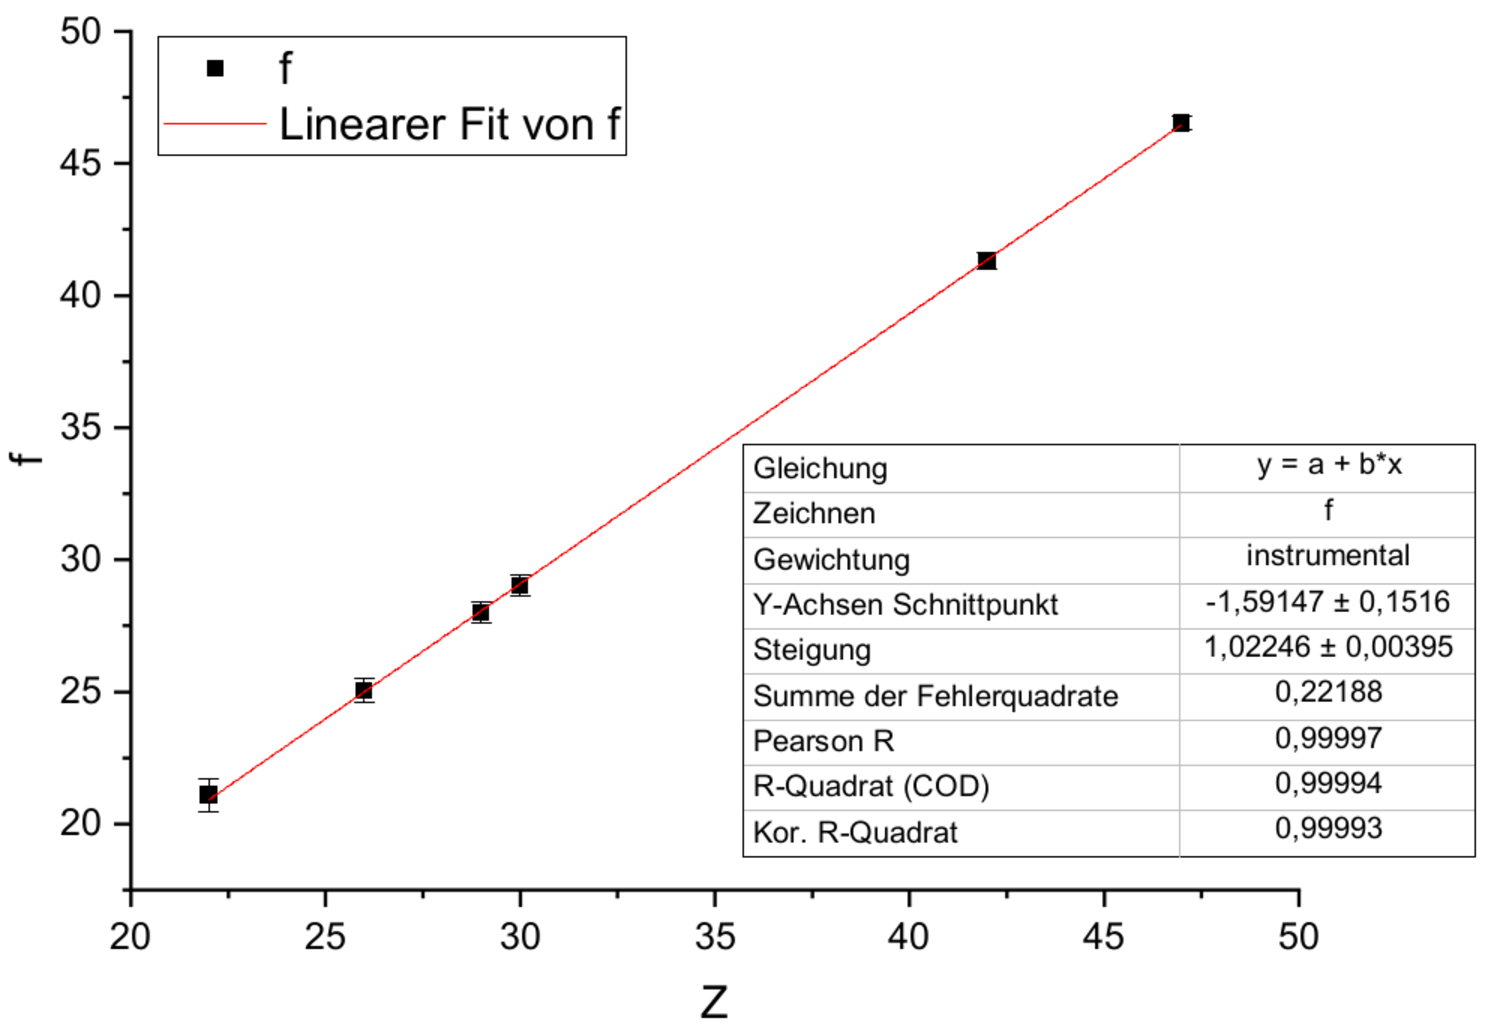
\includegraphics[width=0.8\textwidth]{Ka}
		\centering
		\caption{Die $\text{K}_\alpha$ Übergangsenergien wurden gemäß \cref{eq_f} umgeformt und gegen die Kernladungszahl $Z$ aufgetragen. Dabei beträgt $n_1=1$ und $n_2=2$.}
		\label{fig_Ka}
		\centering
	\end{figure}

	\begin{figure}[H]
		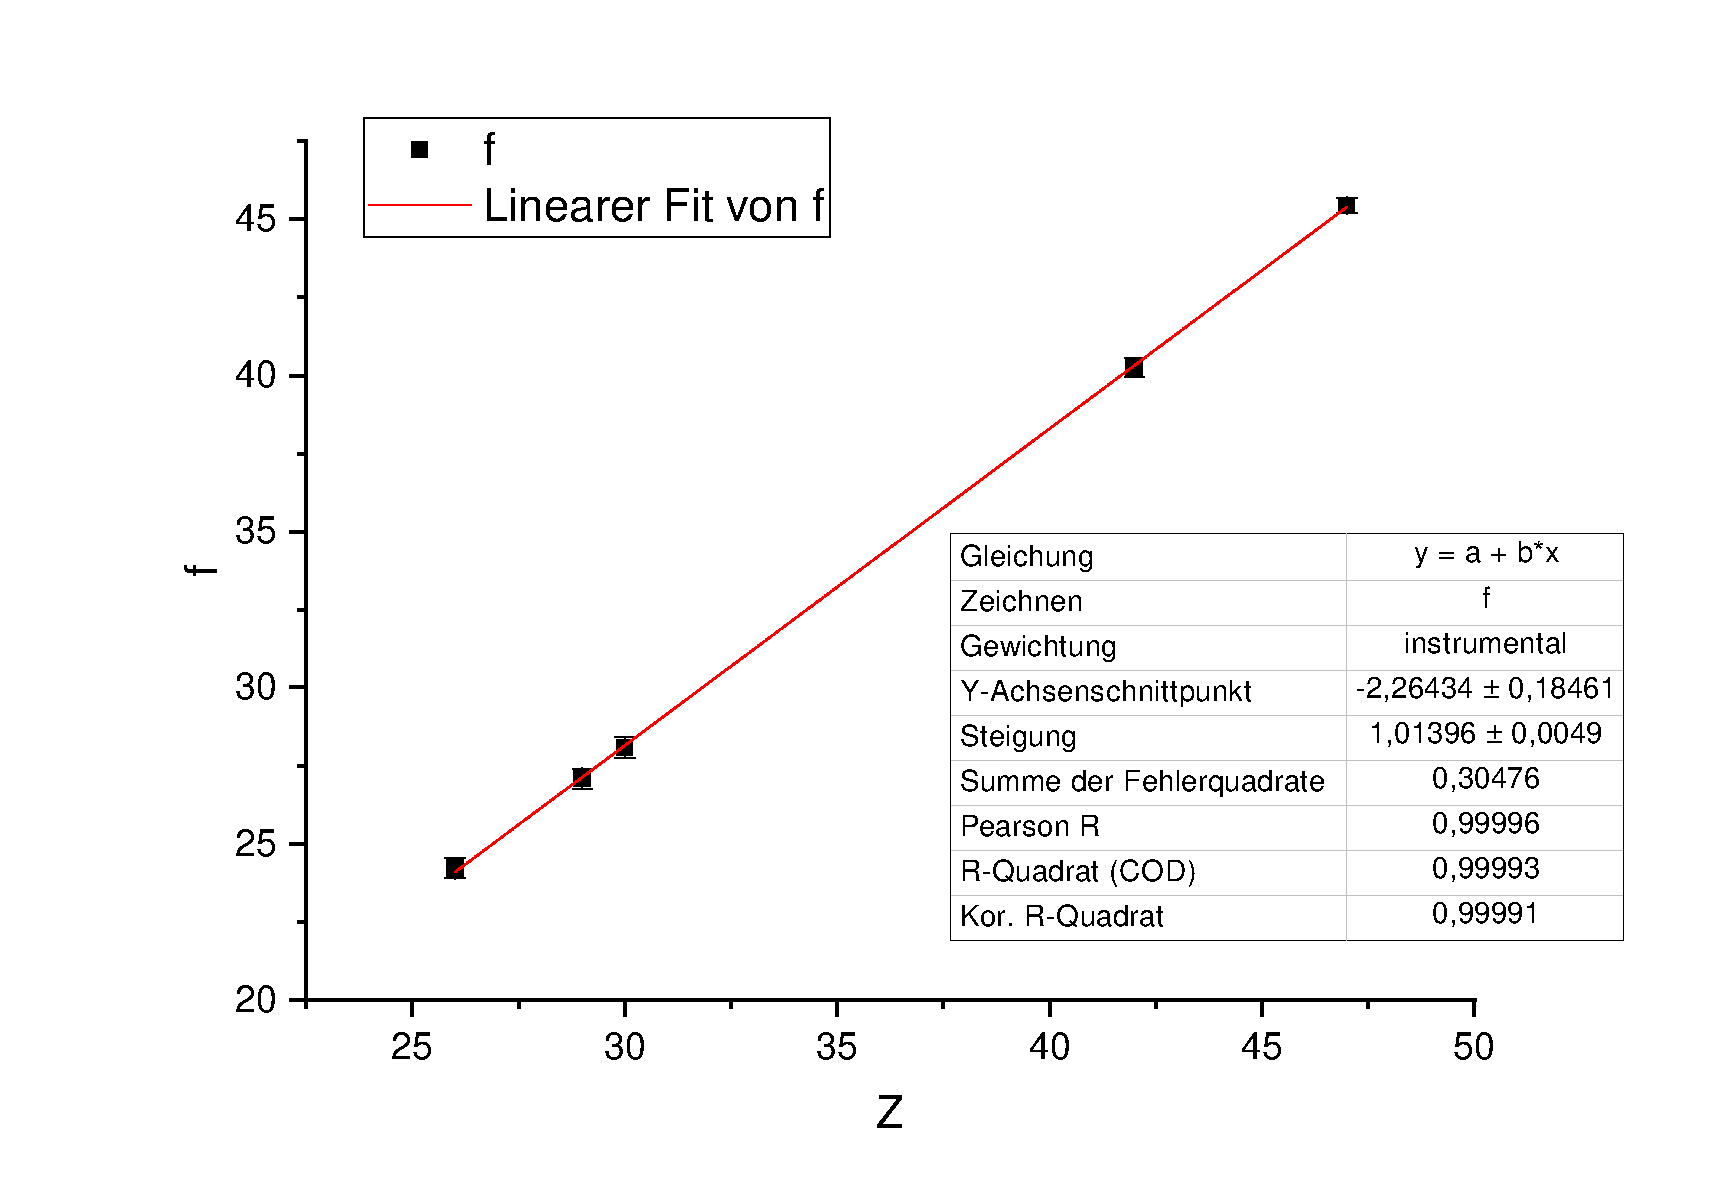
\includegraphics[width=0.8\textwidth]{Kb}
		\centering
		\caption{Die $\text{K}_\beta$ Übergangsenergien wurden gemäß \cref{eq_f} umgeformt und gegen die Kernladungszahl $Z$ aufgetragen. Dabei beträgt $n_1=1$ und $n_2=3$.}
			\label{fig_Kb}
			\centering
	\end{figure}

	Die y-Achsenabschnitte entsprechen $a=-\sigma_{n21}$ und sind die über alle Messpunkte gemittelte Abschirmkonstante.
	Anstelle derer bietet es sich an $\sigma_{n21}$ einzeln zu berechnen, da sie sich mit der Kernladungszahl $Z$ ändert.
	Die Ergebnisse von $\sigma_{n21}=Z-f$ sind in \cref{tb_abschirm} aufgeführt.

	\begin{table}[H] %TODO "Vgl. mit Literaturwerten bietet sich an."
		\centering
		\begin{tabular}{ c | c | c | c | c}
			Element & $\sigma_{n21}$ ($\text{K}_\alpha$) &  $\sigma_{n21}$  ($\text{K}_\beta$) & $\sigma_{n21,\text{Lit}}$($\text{K}_\alpha$)  & $\sigma_{n21,\text{Lit}}$($\text{K}_\beta$) \\ \hline \hline     %TODO angeblicher Rechteschreibfehler
			Ti & \SI{0,90249+-0,31398}{} & - & \SI{0.97039+-0.00003}{}&-\\
			Fe & \SI{0,96914+-0,23049}{} & \SI{1,7825+-0,16282}{} &\SI{0.96860+-0,00002}{}&\SI{1.8369+-0,0002}{}\\
			Cu & \SI{0,99347+-0,20442}{} & \SI{1,90376+-0,15987}{}&\SI{0,945708+-0,000005}{}&\SI{1.85850+-0,00006}{} \\
			Zn & \SI{0.98337+-0.19702}{} & \SI{1.91847+-0.1631}{}&\SI{0,9365+-0,0001}{}&\SI{1.8610+-0,0003}{} \\
			Mo & \SI{0,71061+-0,15659}{} & \SI{1,75324+-0,14985}{} &\SI{0,7282+-0,0003}{}&\SI{1.7444+-0.0004}{}\\
			Ag & \SI{0,48772+-0,13041}{} & \SI{1,56051+-0,12030}{} &\SI{0.5682+-0.0001}{}&\SI{1.5770+-0.0003}{} \\ %TODO text zu Lit in Diskussion
		\end{tabular}
	\caption{Die nach dem Moseleyschen Gesetz bestimmten Abschirmkonstanten der gemessenen $\text{K}_\alpha$ bzw. $\text{K}_\beta$ Übergänge. Die Literaturwerte berechnen sich trivial aus \cref{eq_f} und $E_\text{NIST}$.}
	\label{tb_abschirm}
	\end{table}

	\subsubsection{Bestimmung der Zusammensetzung}
	Die Daten zu den aufgenommenen Peaks sind in \cref{tb_peaks_unknown} mit Vergleichsenergien aufgelistet.
	\begin{table}[H]
		\centering
		\resizebox{\textwidth}{!}{
		\begin{tabular}{ c | c | c || c | c | c }
			Probe (Angabe)&Energie $E_\text{Mess}$ in \SI{}{keV} & rel. &  vermt.& char. &  Energie $E_\text{NIST}$ in \SI{}{keV} \\
			&& Höhe&Element &Übergang & \\
			\hline \hline

			4 (20 Cent)
			& \SI{7.98262+-0.112034}{} &\SI{84}{\%}&Cu &$\text{K}_\alpha$&   \SI{8. 0278416(26) }{} \\
			& \SI{8.7734+-0.123854}{} &\SI{16}{\%}&Cu &$\text{K}_\beta$&  \SI{8 .905413(38) }{} \\
			\hline

			5 (Zn-Edelstahl)
			& \SI{6.41683+-0.178065}{} &\SI{7}{\%}&Fe&K$_\alpha$& \SI{6.3910264(99)}{} \\
			& \SI{8.5778+-0.126318}{} &\SI{80}{\%}&Zn &$\text{K}_\alpha$&  \SI{8.615823(73)}{} \\
			& \SI{9.53652+-0.114435}{} &\SI{12}{\%}&Zn &$\text{K}_\beta$ &  \SI{9.57203(22)}{}  \\
			\hline

			6 (Edelstahl)
			& \SI{3.39677+-0.189573}{} &\SI{1}{\%}&Sn& L$_\alpha$  &  \SI{3 .437356(56) }{} \\
			& \SI{6.36975+-0.123004}{} &\SI{86}{\%}& Fe & $\text{K}_\alpha$ &  \SI{6.3910264(99)}{}  \\
			& \SI{7.07128+-0.101517}{} &\SI{13}{\%}&Fe& $\text{K}_\beta$&  \SI{7.058175(99)}{} \\
			\hline

			9
			& \SI{6.36714+-0.148707}{} &\SI{6}{\%}&Fe &K$_\alpha$& \SI{6.3910264(99)}{} \\
			& \SI{8.57041+-0.12301}{} &\SI{80}{\%}&Zn &$\text{K}_\alpha$&  \SI{8.615823(73)}{}  \\
			& \SI{9.52768+-0.109148}{} &\SI{13}{\%}&Zn &$\text{K}_\beta$ &  \SI{9.57203(22)}{} \\
			\hline

			10
			& \SI{7.4251+-0.121503}{} &\SI{86}{\%}&Ni & K$_\alpha$&  \SI{ 7. 4610343(45)     	}{} \\
			& \SI{8.23717+-0.106367}{} &\SI{14}{\%}&Ni &K$_\beta$&  \SI{ 8. 264775(17)    }{} \\
			\hline

			11 %TODO vmtl. eher Nickel und Kupfer
			& \SI{5.92928+-0.227907}{} &\SI{2}{\%}&Ho & L$_\alpha$&  \SI{ 5. 939963(71)}{} \\
			& \SI{7.79736+-0.202443}{} &\SI{93}{\%}&Ho & L$_\beta$& \SI{7 .76352(49) }{} \\
			& \SI{9.00316+-0.0822221}{} &\SI{5}{\%}&Ho & L$_\beta$& \SI{9 .0511(20) }{} \\
			\hline

			12
			& \SI{9.11464+-0.188139}{} &\SI{4}{\%}&Pb &L$_\alpha$&  \SI{9 .18456(70)    }{} \\
			& \SI{10.5011+-0.130522}{} &\SI{54}{\%}&Pb &L$_\alpha$&  \SI{10. 55160(27)     }{} \\
			& \SI{12.562+-0.144569}{} &\SI{39}{\%}&Pb &L$_\beta$&  \SI{ 12 .6012(13)     }{} \\
			& \SI{14.7821+-0.182134}{} &\SI{4}{\%}&Pb &L$_\beta$&  \SI{  14 .7915(52)    }{} \\
			\hline

			13 %TODO Kupfer+Yttrium+Barium ergibt nen Supraleiter, der bekannt ist => Diskussion?!
			& \SI{4.7454+-0.240256}{} &\SI{10}{\%}& Ba & $\text{L}_\alpha$ & \SI{4. 82758(14)}{} \\
			& \SI{8.00052+-0.126315}{} &\SI{52}{\%}& Cu & $\text{K}_\alpha$ &  \SI{8,0278416(26)}{}\\
			& \SI{8.88531+-0.123469}{} &\SI{9}{\%}& Cu &  $\text{K}_\beta$ & \SI{8,905413(38)}{}\\
			& \SI{14.8774+-0.13453}{} &\SI{24}{\%}& Y & $\text{K}_\alpha$ & \SI{14,88294(26)}{} \\
			& \SI{16.7011+-0.148831}{} &\SI{4}{\%}& Y & $\text{K}_\beta$ &  \SI{16,6447(12)}{} \\
			\hline

			14
			& \SI{3.07729+-0.16356}{} &\SI{9}{\%}&Ag &  $\text{L}_\alpha$ &  \SI{3,150974(36) }{} \\
			& \SI{7.7277+-0.263332}{} &\SI{5}{\%}& Co & $\text{K}_\beta$ &  \SI{7,70598(21)}{} \\
			& \SI{11.8938+-0.238067}{} &\SI{7}{\%}& Au & $\text{L}_\beta $ & \SI{11,8287(14) }{} \\
			& \SI{15.0918+-0.31842}{} &\SI{3}{\%}& Pb & $\text{L}_\beta $ &  \SI{15,1014(54)}{} \\
			& \SI{18.1496+-0.443069}{} &\SI{2}{\%}& Zr & $\text{L}_\gamma $ &  \SI{17,9943(19)}{} \\
			& \SI{22.0709+-0.141621}{} &\SI{65}{\%}&Ag & $\text{K}_\alpha$ &  \SI{21,99030(10)}{} \\
			& \SI{24.9643+-0.16706}{} &\SI{10}{\%}&Ag & $\text{K}_\beta$ &  \SI{24,94242(30)}{} \\
			\hline

			15
			& \SI{7.99436+-0.125916}{} &\SI{86}{\%}& Cu & $\text{K}_\alpha$ &  \SI{8,0278416(26)}{} \\
			& \SI{8.88485+-0.109037}{} &\SI{14}{\%}&  Cu &  $\text{K}_\beta$ & \SI{8,905413(38)}{} \\
			\hline

			16 (1-Cent)
			& \SI{7.98818+-0.117498}{} &\SI{86}{\%}& Cu & $\text{K}_\alpha$ &  \SI{8,0278416(26)}{} \\
			& \SI{8.8637+-0.107308}{} &\SI{14}{\%}& Cu &  $\text{K}_\beta$ & \SI{8,905413(38)}{} \\
			\hline

			17
			& \SI{7.98377+-0.112928}{} &\SI{86}{\%}& Cu & $\text{K}_\alpha$ & \SI{8,0278416(26)}{} \\
			& \SI{8.85058+-0.106618}{} &\SI{14}{\%}& Cu & $\text{K}_\beta$ & \SI{8,905413(38)}{} \\
			\hline

			18
			& \SI{7.41993+-0.114157}{} &\SI{86}{\%}& Ni & $\text{K}_\alpha$ & \SI{7,4610343(45)}{} \\
			& \SI{8.21747+-0.102606}{} &\SI{14}{\%}& Ni & $\text{K}_\beta$ &   \SI{8,264775(17)}{} \\
			\hline

			19
			& \SI{5.40493+-0.124428}{} &\SI{31}{\%}& Cr & $\text{K}_\alpha$ & \SI{5,4055384(71)}{} \\
			& \SI{6.33056+-0.11387}{} &\SI{59}{\%}& Fe & $\text{K}_\alpha$ & \SI{ 6,3910264(99)}{} \\
			& \SI{7.05903+-0.217815}{} &\SI{10}{\%}& Fe &  $\text{K}_\beta $ & \SI{7,058175(16)}{} \\
			\hline

			20 (Kronkorken)
			& \SI{4.52319+-0.152823}{} &\SI{4}{\%}& Ti & $\text{K}_\alpha $ &  \SI{4. 5108991(94)}{} \\
			& \SI{6.35883+-0.11196}{} &\SI{83}{\%}& Fe & $\text{K}_\alpha $ &  \SI{6,3910264(99)}{} \\
			& \SI{7.03423+-0.103302}{} &\SI{13}{\%}& Fe & $\text{K}_\beta $ &  \SI{7,058175(16)}{} \\
			\hline
		\end{tabular}
		}
		\caption{Gemessene Röntgenfluoreszenzmaxima. Die charakteristischen Übergangsenergien sind die experimentellen Werte aus \cite{XRAYDB}.
		Es gibt bei Probe 11 und 12 mehrfach gleichnamige Übergänge, da verschiedene Orbitale gleicher Schale unterschiedliche Energieniveaus haben.}
		\label{tb_peaks_unknown}

	\end{table}

	Um mit \cref{eq_anteil} die Massenteile $C_i$ eines Elements in der Probe bestimmen zu können ist es notwendig, dass alle Peaks einem Referenz-Spektrum ($H_{0i}$) zugeordnet werden können.
	Bei den Proben aus \cref{tb_peaks_unknown} mit \cref{tb_peaks_known} als Referenz-Spektrum ist dies lediglich für Probe 20, den Kronkorken, möglich.

	\begin{equation}
		\label{eq_anteil}
		C_j = \frac{\rho_i \cdot \frac{H_j}{H_{0j}}}{\sum_{i} \rho_i \cdot \frac{H_i}{H_{0i}}}
	\end{equation}

	Die Unsicherheiten der Dichten $\rho_\text{Fe}=\SI{7.874}{g/cm^3}$ und $\rho_\text{Ti}=\SI{4.540}{g/cm^3}$ verschwinden gegenüber denen der Peakhöhen, welche mit 5\% abgeschätzt werden. \cite{density}
	In \cref{tb_peaks} sind die für zum Berechnen benötigen Messwerte aufgeführt.

	\begin{table}[H]
		\centering
		\begin{tabular}{ c | c }
			 & Höhe in a.u.\\ \hline \hline
			$H_{0 , \text{Fe}}$ & \SI{2737.86+-136.89}{} \\
			$H_{\text{Fe}}$ & \SI{1899.26+-84.96}{} \\
			$H_{0 , \text{Fe}}'$ & \SI{414.38+-20.72}{} \\
			$H_{\text{Fe}}'$ & \SI{157.24+-7.86}{} \\
			$H_{0 , \text{Ti}}$ & \SI{1136.09+-56.80}{} \\
			$H_{\text{Ti}}$ & \SI{82.82+-4.14}{} \\
		\end{tabular}
		\caption{Höhen der Referenz- und Probenpeaks von Eisen und Titan.} %TODO mehr
		\label{tb_peaks}
	\end{table}

	\begin{equation}
		\label{eq_anteil_calc}
		1-C_\text{Ti}= C_\text{Fe} = \frac{1}{1+ \frac{\rho_\text{Ti} H_\text{Ti} H_{0,\text{Fe}}}{\rho_\text{Fe} H_\text{Fe} H_{0,\text{Ti}}}}
	\end{equation}

	Einsetzen in \cref{eq_anteil_calc} ergibt $C_\text{Fe}=\SI{94.3+-0.5}{\%}$ und $C_\text{Ti}=\SI{5.7+-0.5}{\%}$, bzw. mit dem kleineren Peak, also $H'$, $C_\text{Fe}'=\SI{94.6+-0.5}{\%}$ und $C_\text{Ti}'=\SI{5.4+-0.5}{\%}$

	\subsection{Diskussion}
	\subsubsection{Bestimmung der Abschirmkonstanten}
	Die gemessenen Energien in \cref{tb_peaks_known} können zum größten Teil charakteristischen Übergängen in den jeweiligen Elementen zugeordnet werden.
	Obwohl die Proben jedoch nicht als Legierung gekennzeichnet sind, treten jedoch im Fall von Probe 1, 2, 7 und 8 Peaks auf, bei denen dies nicht möglich ist.
	Hier steht zu vermuten, dass in geringen Mengen andere Elemente beigemischt wurden, von denen aber jeweils nur der häufigste Übergang messbar ist, weshalb sie nicht eindeutig identifiziert werden können.

	Das Moseleysche Gesetz kann insofern bestätigt werden, als dass die Steigungen in \crefrange{fig_Ka}{fig_Kb} gemäß der vorgenommenen Näherung nahe an \num{1} liegt.
	Die Abweichung nach oben hängt vermutlich mit der Tatsache zusammen, dass die mittlere Abschirmkonstante mit der Kernladungszahl abnimmt.
	Dies spiegelt sich auch in \cref{tb_abschirm} wieder, wobei hier die große Unsicherheit eine präzisere Aussage unmöglich macht.
	%TODO Abweichung vom Fit diskutieren: 1,5 im Vergleich zu <1 (sigma_n21 ist wohl gemeint)
	Der Vergleich mit den berechneten Abschirmkonstanten lässt feststellen, dass die gemessenen Werte immer leicht unter den jenen liegen, aber die berechneten Abschirmkonstanten immer innerhalb der Unsicherheit der Messwerte liegen.
	%TODO ich schätze, ich sollte hier noch was sagen, warum das so ist, aber kp, was das sein könnte.

	\subsubsection{Bestimmung der Zusammensetzung}
	Zunächst ist bei den Proben eigentlich bekannter Zusammensetzung (\cref{tb_peaks_known}) festzustellen, dass offenbar teilweise verunreinigte Proben vorliegen.
	So kann bei Probe 1 (Zink) die $\text{K}_\alpha$-Linie von Eisen und bei Probe 2 (Eisen) die $\text{L}_\alpha$-Linie von Zinn gemessen werden.

	Bei Probe 7 (Titan) ist ebenfalls die  $\text{K}_\alpha$-Linie von Eisen sichtbar.
	Zusätzlich tritt ein Peak auf, bei dem vermutet werden kann, dass er die Überlagerung des $\text{L}_\alpha$-Übergangs von Molybdän und des $\text{L}_\beta$-Übergangs von Zirconium ist.
	Außerdem wurde hier ein Peak bei \SI{1,392}{keV} gemessen.
	Dies liegt außerhalb des Messbereichs des Röntgendetektors, weshalb der Peak nicht weiter betrachtet wird.

	Bei Probe 8 (Molybdän) wird ein Übergang gemessen, der der Überlagerung der $\text{K}_\alpha$-Übergänge von Nickel und Kupfer zugeschrieben werden kann und ein weiterer, der beim $\text{K}_\alpha$-Übergang von Selen liegt.

	Diese Verunreinigungen sind insofern nachteilhaft, als dass sie die Bestimmung der Massenanteile der anderen Proben weniger zuverlässig machen, für die reine Proben nötig sind.

	Die Bestimmung der Zusammensetzung der unbekannten Proben ist teilweise mit großer Sicherheit möglich, teilweise jedoch dadurch erschwert, dass mehrere Elemente in Frage kommen und die Unsicherheit der Messwerte sehr groß ist.
	Es werden die Energien und relativen Höhen der gemessenen Peaks in \cref{tb_peaks_unknown} mit denen der bekannten Proben aus \cref{tb_peaks_known} sowie den Angaben aus \cite{XRAYDB} verglichen.
	Da dies häufig noch mehrere Möglichkeiten für die Zusammensetzung offen ließ, werden zusätzliche Annahmen darüber getroffen, welche Elemente auf Basis des Aussehens der Proben wahrscheinlich sind.
	Auch dies führt jedoch nicht in allen Fällen zu einer eindeutigen Bestimmung der Bestandteile der Proben.
	Damit ergibt sich:

	\begin{enumerate}
		\item[Probe 4] Hier kann recht eindeutig Kupfer als Hauptbestandteil identifiziert werden. Dies stimmt mit den Erwartungen überein, da 20-Cent-Münzen aus nordischem Gold bestehen (vgl. \cite{muenzen}), welches zu 89\% aus Kupfer besteht. Die anderen Anteile (5\% Zink, 5\% Aluminium. 1\% Zinn) konnten nicht identifiziert werden. Dies ist eine wichtige Feststellung für die Limitierungen dieses Verfahrens.
		\item[Probe 5] Hier kann Zink als Hauptbestandteil festgestellt werden. Es fällt allerdings auf, dass zusätzlich ein Peak mit 7\% relativer Höhe auftritt, der keinem Übergang im Zink-Atom zugeordnet werden kann. Die Energie des Peaks entspricht dem $\text{K}_\alpha$-Übergang in Eisen. Dies war allerdings bereits bei Probe 1 der Fall, obwohl diese als (reines) Zink gekennzeichnet ist. Das lässt die Schlussfolgerung zu, dass in beiden Fällen Eisen beigemischt ist. Dies würde die Angabe zu Probe 5 bestätigen, da diese sie als Zn-Edelstahl bezeichnet hat.
		\item[Probe 6] Probe 6 sollte laut Angabe Edelstahl sein. Dies kann bestätigt werden, da die gleichen Übergänge wie in Probe 2 (Fe) auftreten. In beiden Fällen tritt jedoch zusätzlich zu den in Eisen charakteristischen Übergängen ein weiterer auf. Hier kann wie zuvor nur vermutete werden, dass entweder in beiden Fällen ein anderes Element beigemischt war oder ein Übergang unerwarteter Energie auftritt.
		\item[Probe 9] Es wurden die gleichen Übergänge wie bei Probe 1 und 5 gemessen. Hauptbestandteil ist Zink. Ansonsten gelten dieselben Überlegungen wie bei Probe 5.
		\item[Probe 10] kann auf Basis der Angaben von \cite{XRAYDB} als Nickel identifiziert werden.
		\item[Probe 11] kann auf Basis der Angaben von \cite{XRAYDB} als Holmium identifiziert werden.
		\item[Probe 12] kann auf Basis der Angaben von \cite{XRAYDB} als Blei identifiziert werden.
		\item[Probe 13] Je zwei Übergänge können Kupfer und Yttrium zugeordnet werden. Der fünfte Übergang ist schwieriger zuzuordnen. Da jedoch Yttrium-Barium-Kupferoxid ein wichtiger Hochtemperatursupraleiter ist, wird angenommen, dass er Barium zugeordnet. %TODO Grund, warum kein sauerstoff gemessen.
		\item[Probe 14] Das Spektrum lässt nur ein eindeutiges Identifizieren von Silber zu. Die vier anderen gemessenen Peaks sind nicht nur einem oder zwei Elementen zuordenbar. Es werden deswegen Elemente gewählt, die passende Übergänge bei diesen Energien haben, auf der Erde vorkommen und stabile Isotope haben. Das Ergebnis lautet Zirconium, Blei, Gold und Cobalt. Dieses Ergebnis ist nicht sehr aussagekräftig, da bei diesen Elementen zu erwarten wäre, dass auch andere Übergänge im Spektrum zu sehen sind. Hier tritt allerdings ein weiteres Problem dieser Methode zutage, da, wenn zwei Übergänge in der Probe energetisch hinreichend nah zusammen fallen, sie nicht mehr im Spektrum unterscheidbar sind.
		\item[Probe 15] kann auf Basis der Messungen in \cref{tb_peaks_known} als Kupfer identifiziert werden.
		\item[Probe 16] kann auf Basis der Messungen in \cref{tb_peaks_known} als Kupfer identifiziert werden. Dies stimmt mit der Erwartung für 1-Cent-Münzen überein, da diese aus mit Kupfer ummanteltem Eisen bestehen. Die Röntgenphotonen dringen offenbar nicht zum Eisen durch bzw. die vom Eisen emittierten Fluoreszenzphotonen dringen nicht durch die Ummantelung zum Detektor vor.%, weshalb  für die Eindringtiefe der Röntgenphotonen in Kupfer gefunden wurde. %TODO kann leider net sagen, was die ist, weil finde ich nicht
		\item[Probe 17] kann auf Basis der Messungen in \cref{tb_peaks_known} als Kupfer identifiziert werden.
		\item[Probe 18] kann auf Basis der Angaben von \cite{XRAYDB} als Nickel identifiziert werden.
		\item[Probe 19] Hier kann recht eindeutig Eisen identifiziert werden. Zusätzlich tritt ein Peak bei einer Energie auf, die dem $\text{K}_\alpha$-Übergang im Chrom entspricht.
		\item[Probe 20] Hier kann recht eindeutig Eisen identifiziert werden. Zusätzlich tritt ein Peak bei einer Energie auf, die dem $\text{K}_\alpha$-Übergang im Titan entspricht. Dies ist kein Element, dass in Kronkorken zu erwarten wäre, aber gemäß der Berechnung der Massenanteile nimmt es lediglich 5\% ein. Da jedoch zuvor schon festgestellt wurde, dass die Eindringtiefe recht gering ist, kann hier die Lackierung des Kronkorkens einen signifikanten Einfluss gehabt haben. Einige Lacke enthalten Titan, was der Grund für das Auftreten dieser Linien sein kann.
	\end{enumerate}

	\section{Schlussfolgerung}
	Es konnten verschiedene Untersuchungen mithilfe von Röntgenspektroskopie gemacht werden.
	Zunächst wurden charakteristische Übergangsenergien von sechs Elementen gemessen und zugeordnet.
	Auf Basis dessen konnte für den größten Teil der anderen Proben mit hoher Sicherheit die Anteile bestimmt werden, die in ausreichender Menge vorhanden sind, damit ihre Peaks im Spektrum sichtbar sind.
	Es wurde jedoch auch offensichtlich, dass die Methode der energiedispersiven Röntgenspektroskopie mit dem verwendeten Röntgengerät keine adäquate Technik ist, um Proben zu analysieren, die entweder aus vielen verschiedenen Elementen bestehen oder um Elementbestandteile zu finden, deren Anteil unter etwa 5\% liegt. % 5% ist bissl willkürlich, aber präziser als so ein Ausdruck wie zu gering
	Außerdem können für eine Probe die Massenbestandteile bestimmt werden.
	Hierbei wurde deutlich, dass die Effektivität dieser Methode massiv mit den vorhandenen Referenzmessungen reiner Proben skaliert, da einige Proben aus Mangel einer solchen Messung nicht auf Massenanteile untersucht werden konnten.

	Obwohl das Moseleysche Gesetz bestätigt werden konnte, kann dieses Verfahren nicht als gut zur Bestimmung der mittleren Abschirmkonstanten geeignet bezeichnet werden, da dies nur mit sehr großen Unsicherheiten möglich war.

	Das Programm, das zur Erfassung der Messdaten des Röntgendetektors verwendet wurde, hat die Messung zusätzlich erschwert, da es insgesamt sieben mal nach abgeschlossener Messung abgestürzt ist, was das Wiederholen der Messung erzwang. Ohne dieses Problem lässt sich sagen, dass längere Messungen die Unsicherheiten deutlich verringern würden.
	Zusätzlich würde eine Röntgenröhre, die mit höherer Spannung betrieben werden kann, es ermöglichen Übergänge größerer Energie zu messen.


	%TODO Längere messung für mehr Präzession für kleine Peaks, bessere Kannone => mehr Photonen?

	\printbibliography

	\section{Anhang}
	%TODO check ob das mit der Tabelle passt ://

	\begin{figure}[H]
		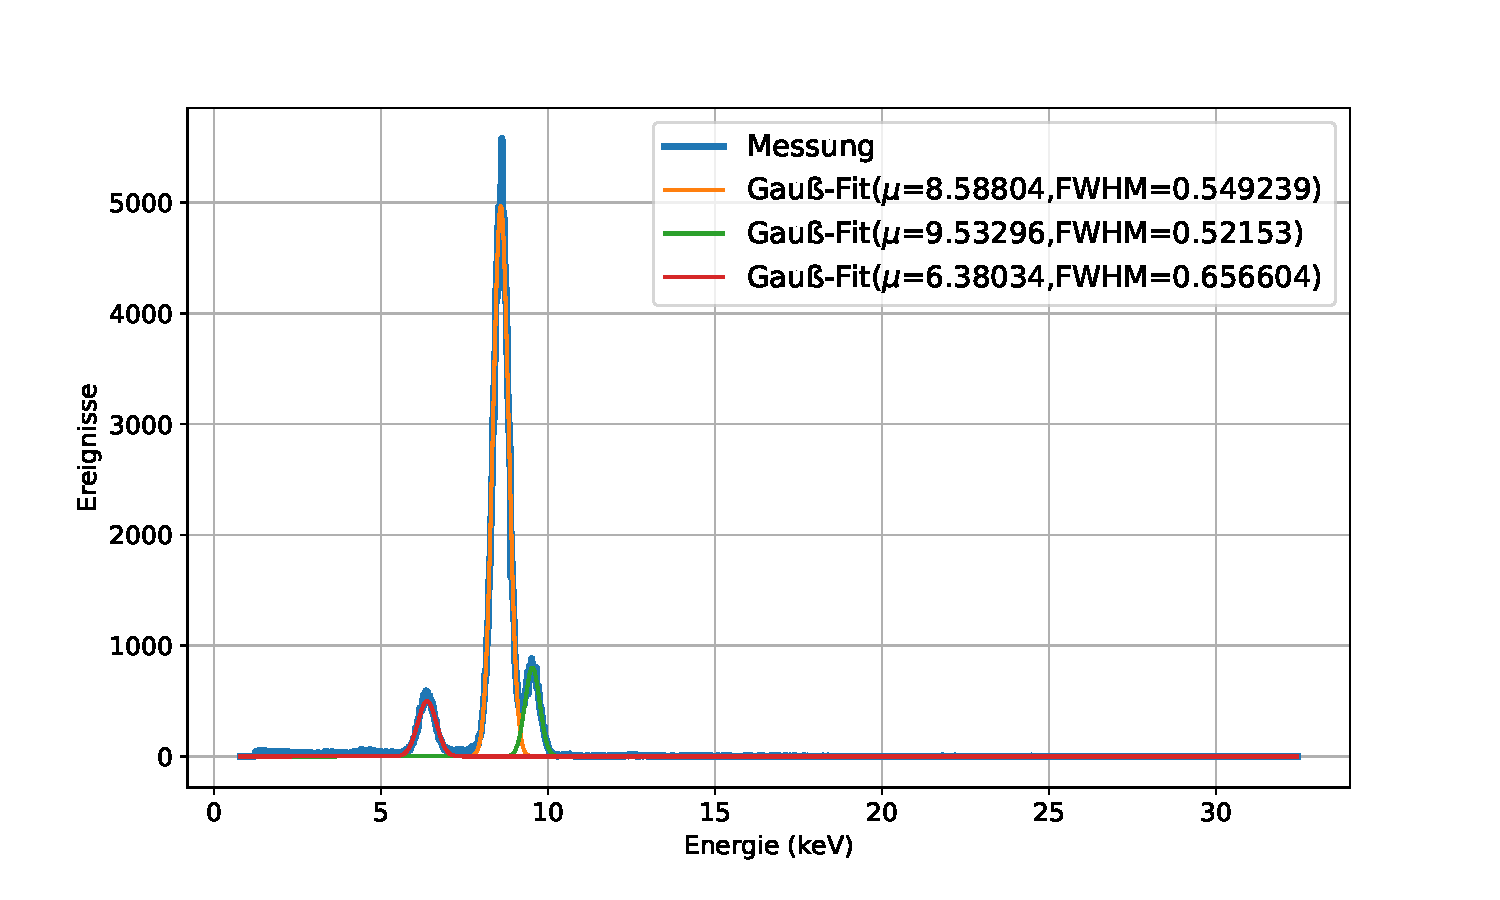
\includegraphics[width=0.95\textwidth]{images/1-Zn.pdf}
		\centering
		\caption{Röntgenfluoreszenzspektrum der Probe 1.}
	\end{figure}

	\begin{figure}[H]
		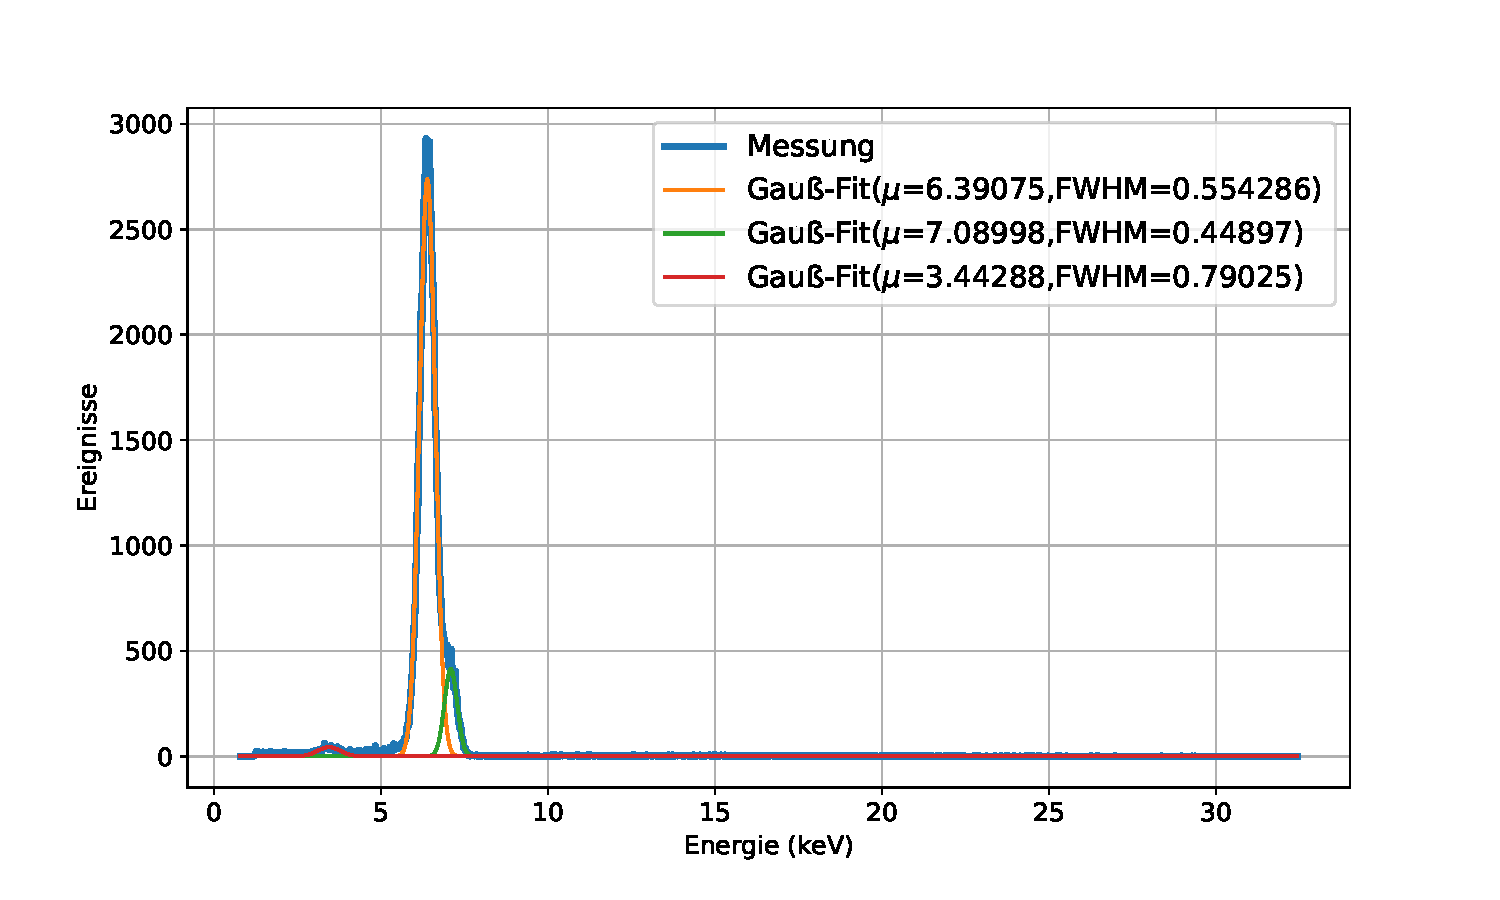
\includegraphics[width=0.95\textwidth]{images/2-Fe.pdf}
		\centering
		\caption{Röntgenfluoreszenzspektrum der Probe 2.}
	\end{figure}

	\begin{figure}[H]
		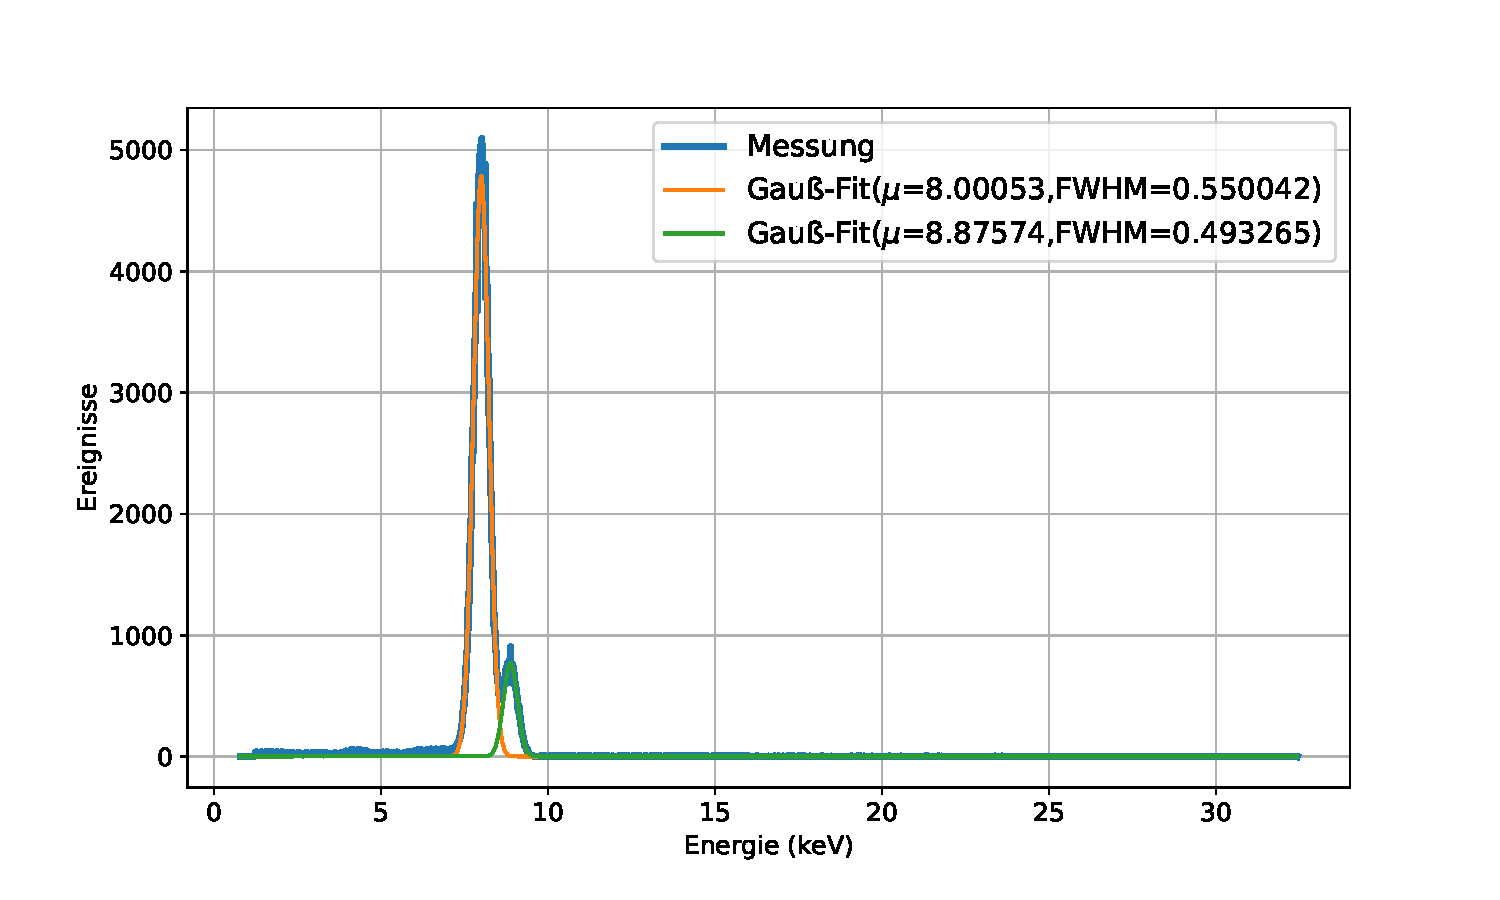
\includegraphics[width=\textwidth]{images/3-Cu.pdf}
		\centering
		\caption{Röntgenfluoreszenzspektrum der Probe 3.}
	\end{figure}

	\begin{figure}[H]
		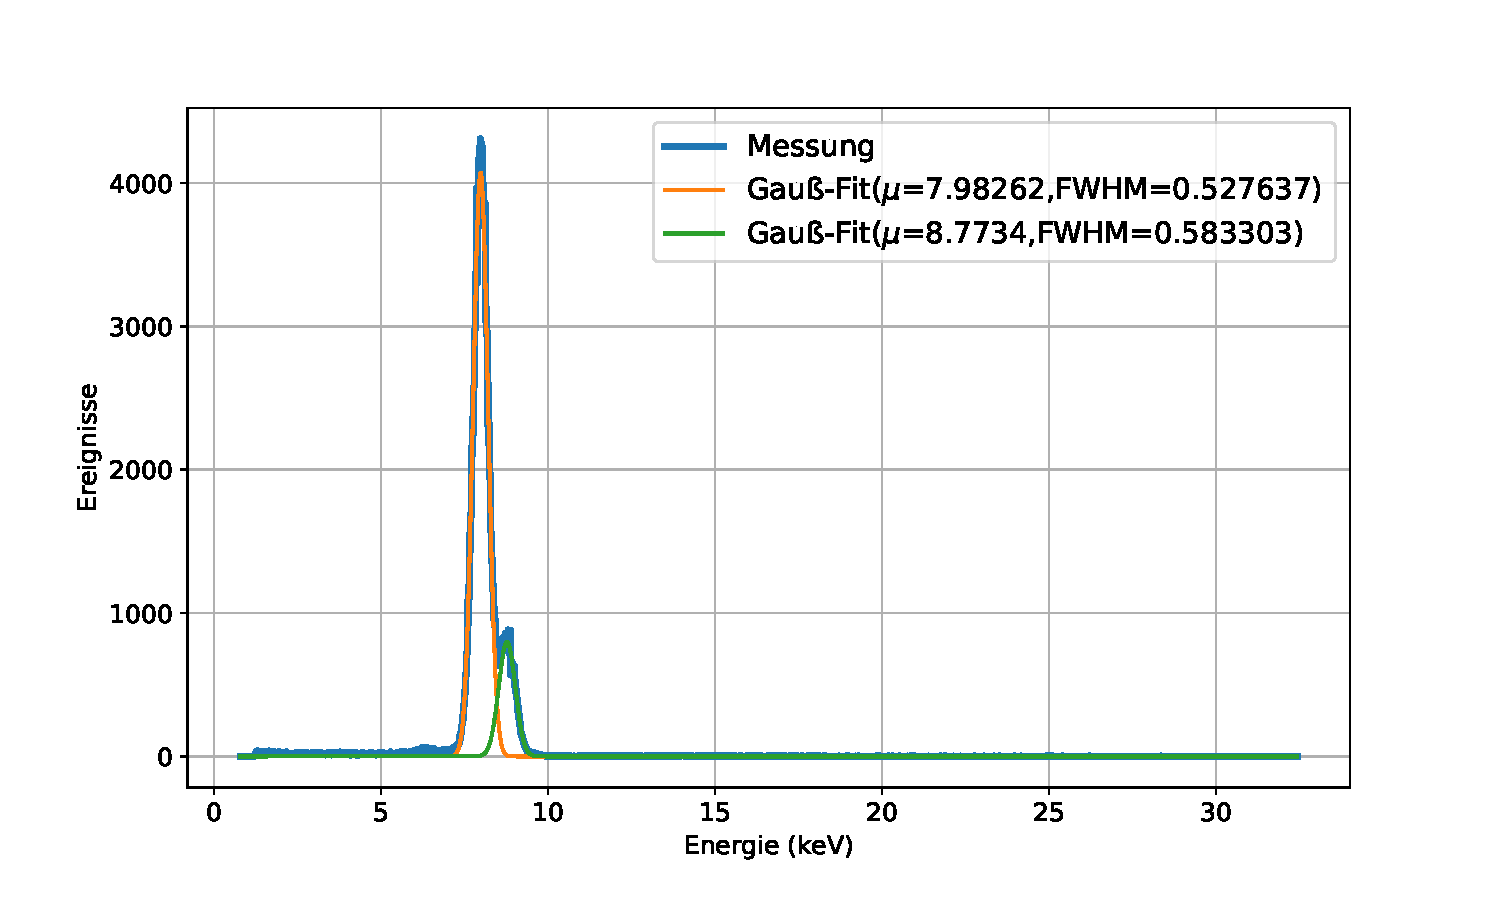
\includegraphics[width=\textwidth]{images/4-20-Cent.pdf}
		\centering
		\caption{Röntgenfluoreszenzspektrum der Probe 4.}
	\end{figure}

	\begin{figure}[H]
		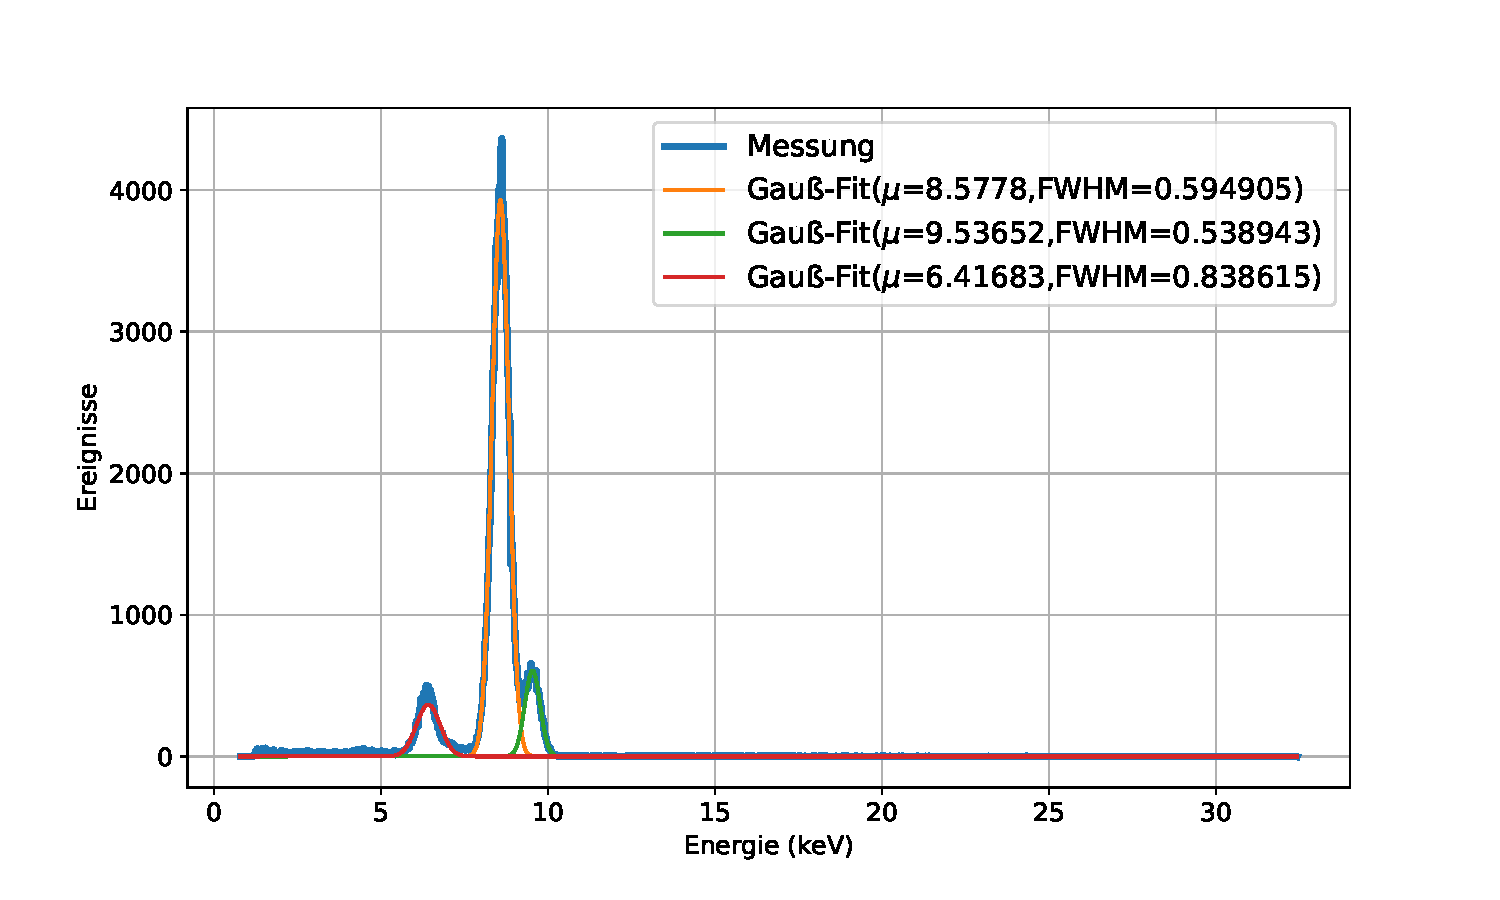
\includegraphics[width=\textwidth]{images/5-Zn-EdelStahl.pdf}
		\centering
		\caption{Röntgenfluoreszenzspektrum der Probe 5.}
	\end{figure}

	\begin{figure}[H]
		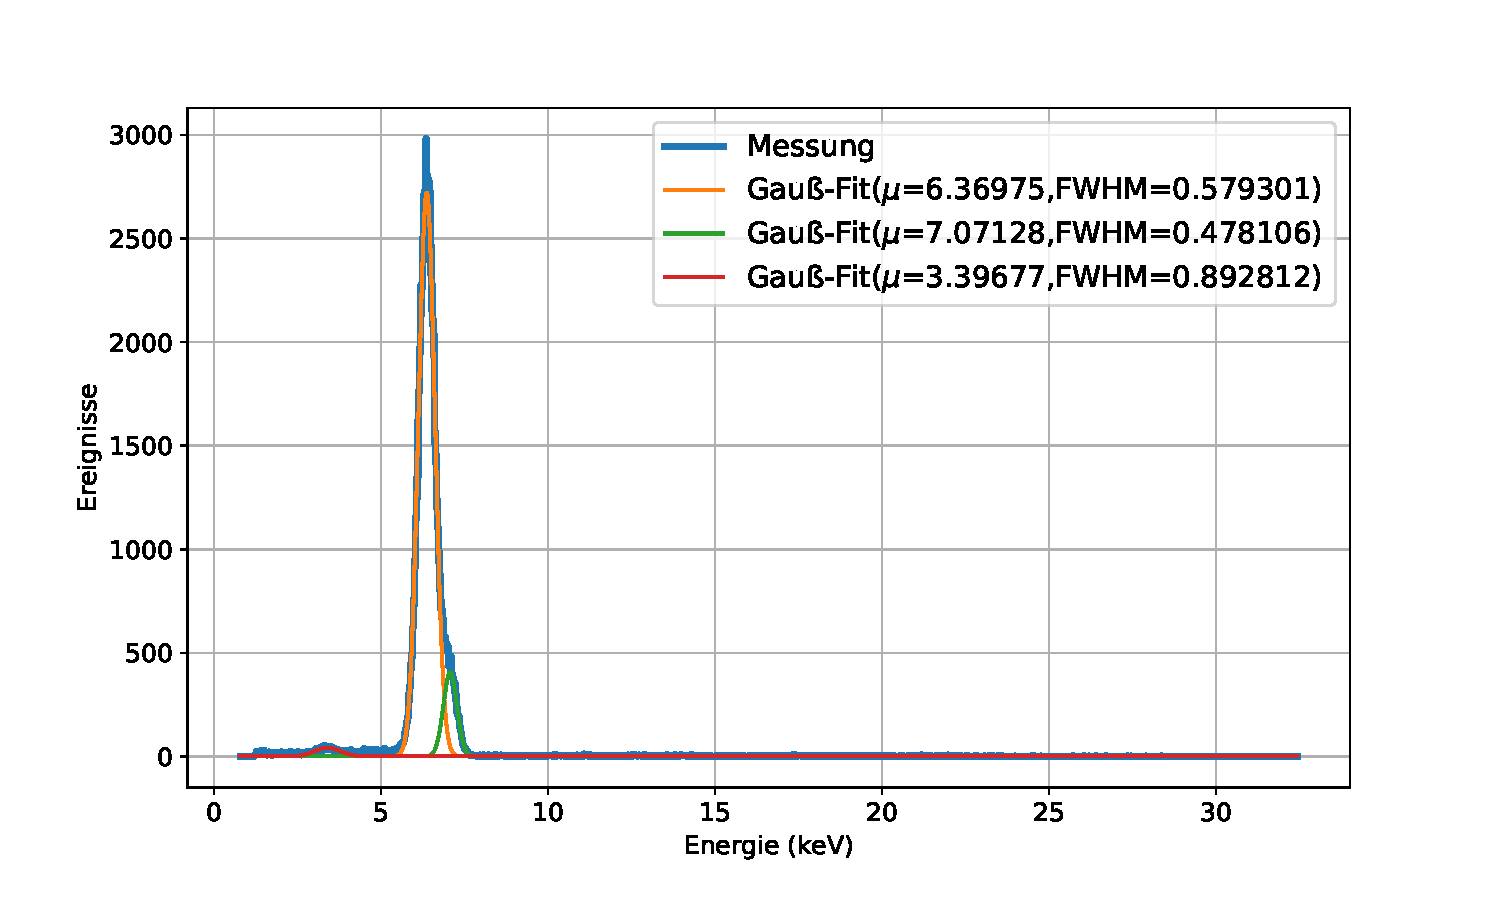
\includegraphics[width=\textwidth]{images/6-EdelStahl.pdf}
		\centering
		\caption{Röntgenfluoreszenzspektrum der Probe 6.}
	\end{figure}

	\begin{figure}[H]
		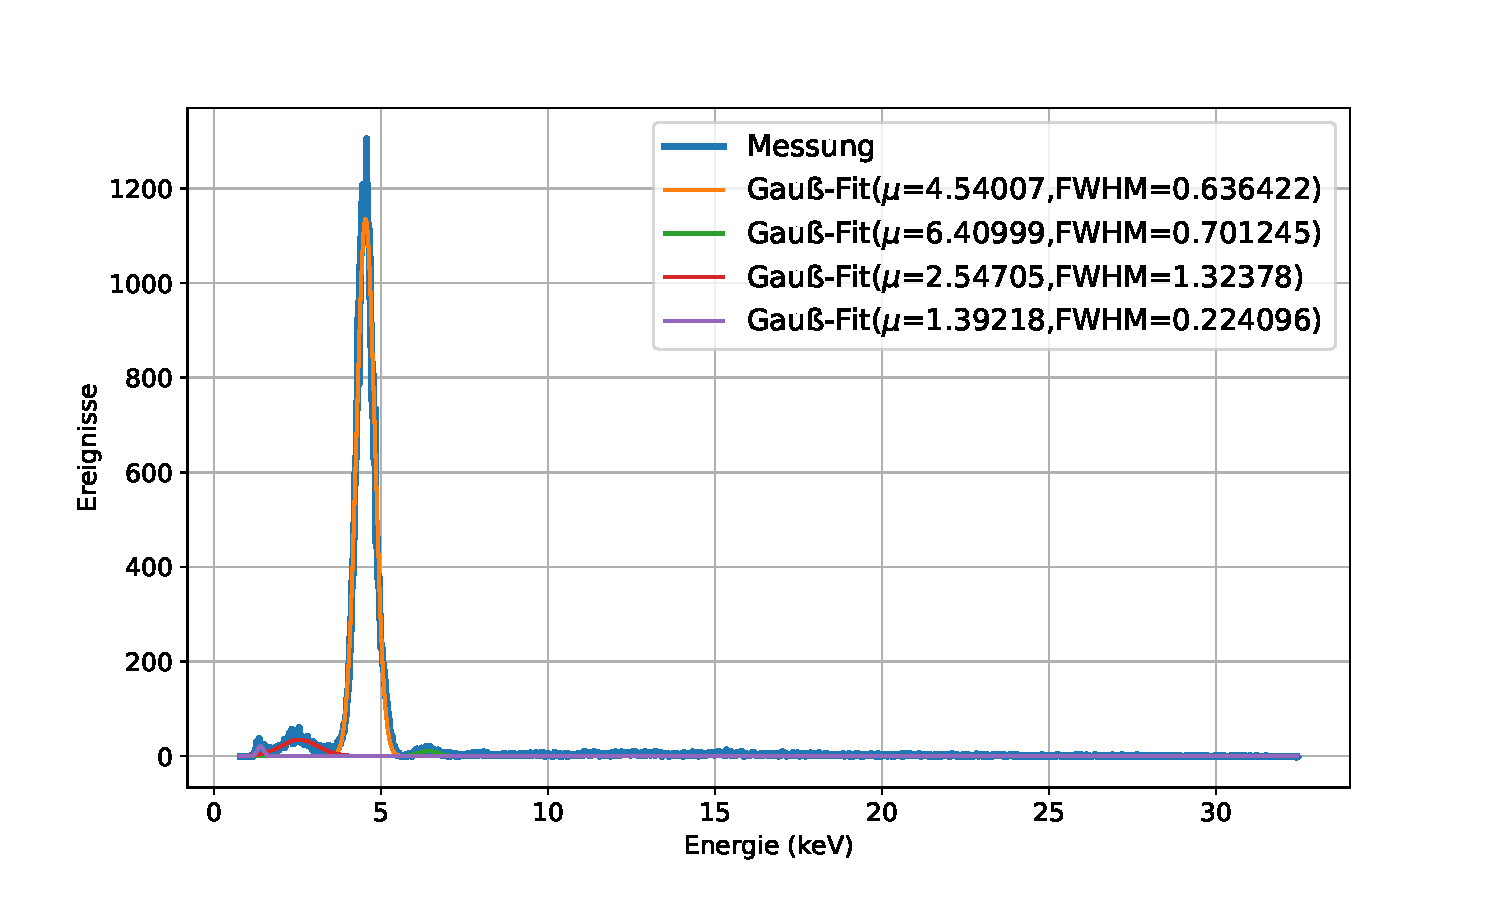
\includegraphics[width=\textwidth]{images/7-Ti.pdf}
		\centering
		\caption{Röntgenfluoreszenzspektrum der Probe 7.}
	\end{figure}

	\begin{figure}[H]
		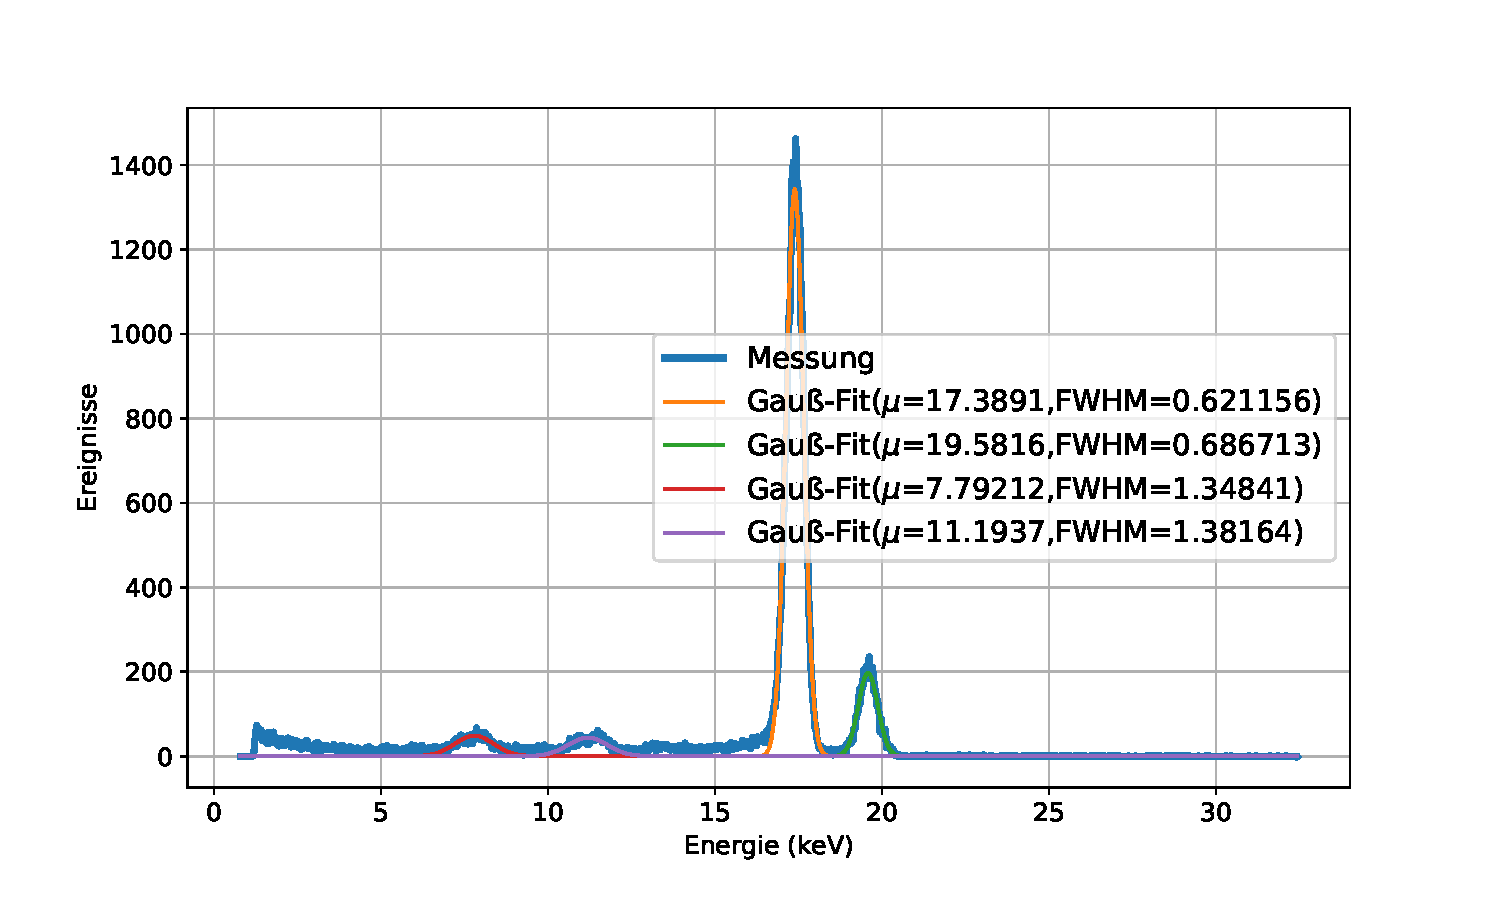
\includegraphics[width=\textwidth]{images/8-Mo.pdf}
		\centering
		\caption{Röntgenfluoreszenzspektrum der Probe 8.}
	\end{figure}

	\begin{figure}[H]
		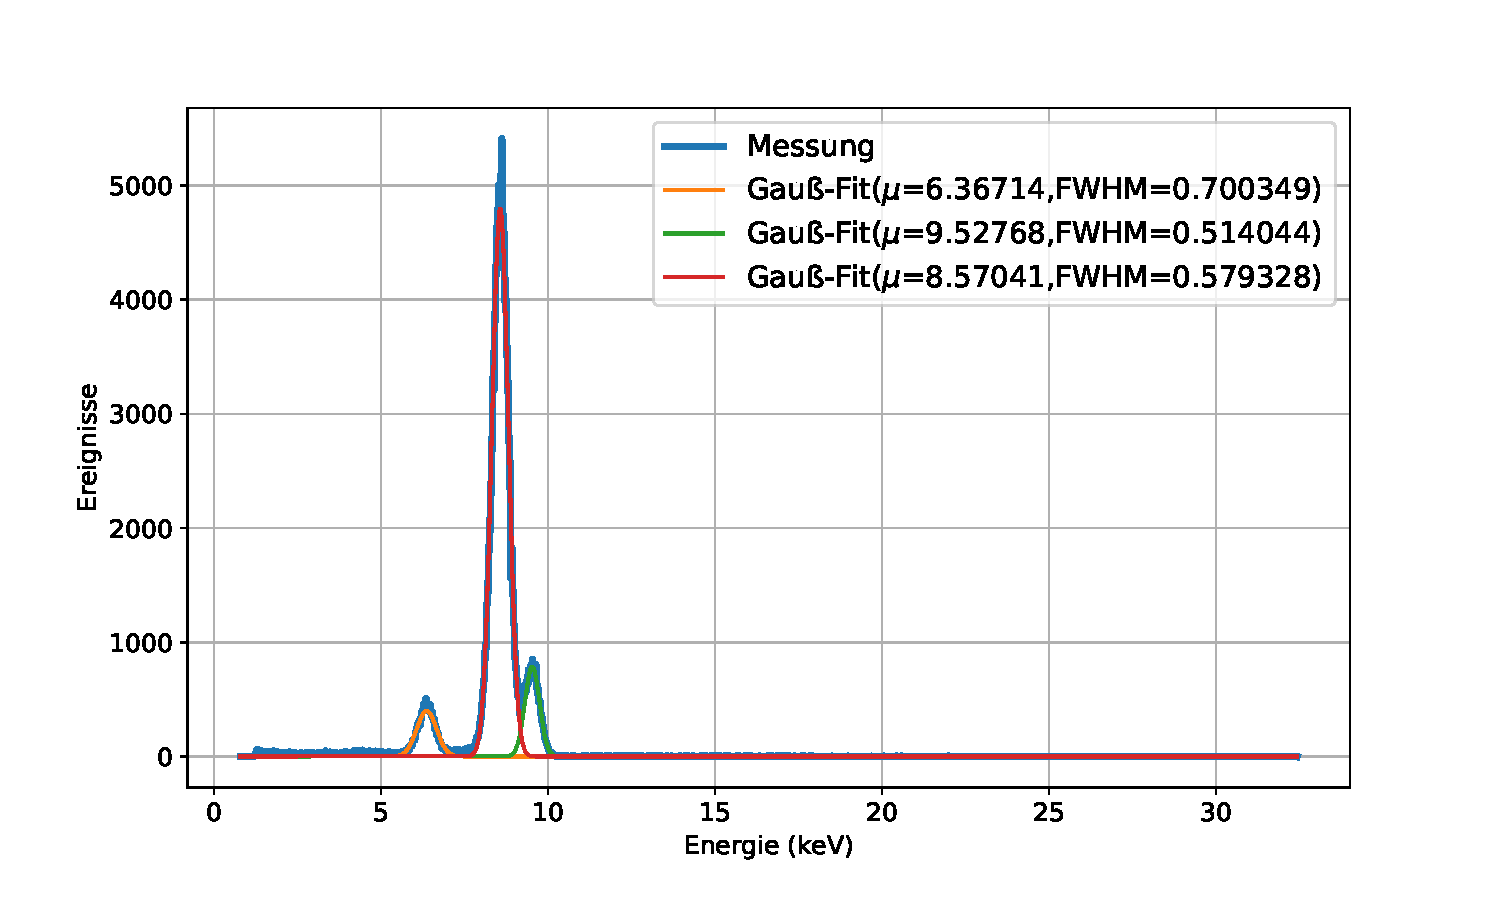
\includegraphics[width=\textwidth]{images/9-X.pdf}
		\centering
		\caption{Röntgenfluoreszenzspektrum der Probe 9.}
	\end{figure}

	\begin{figure}[H]
		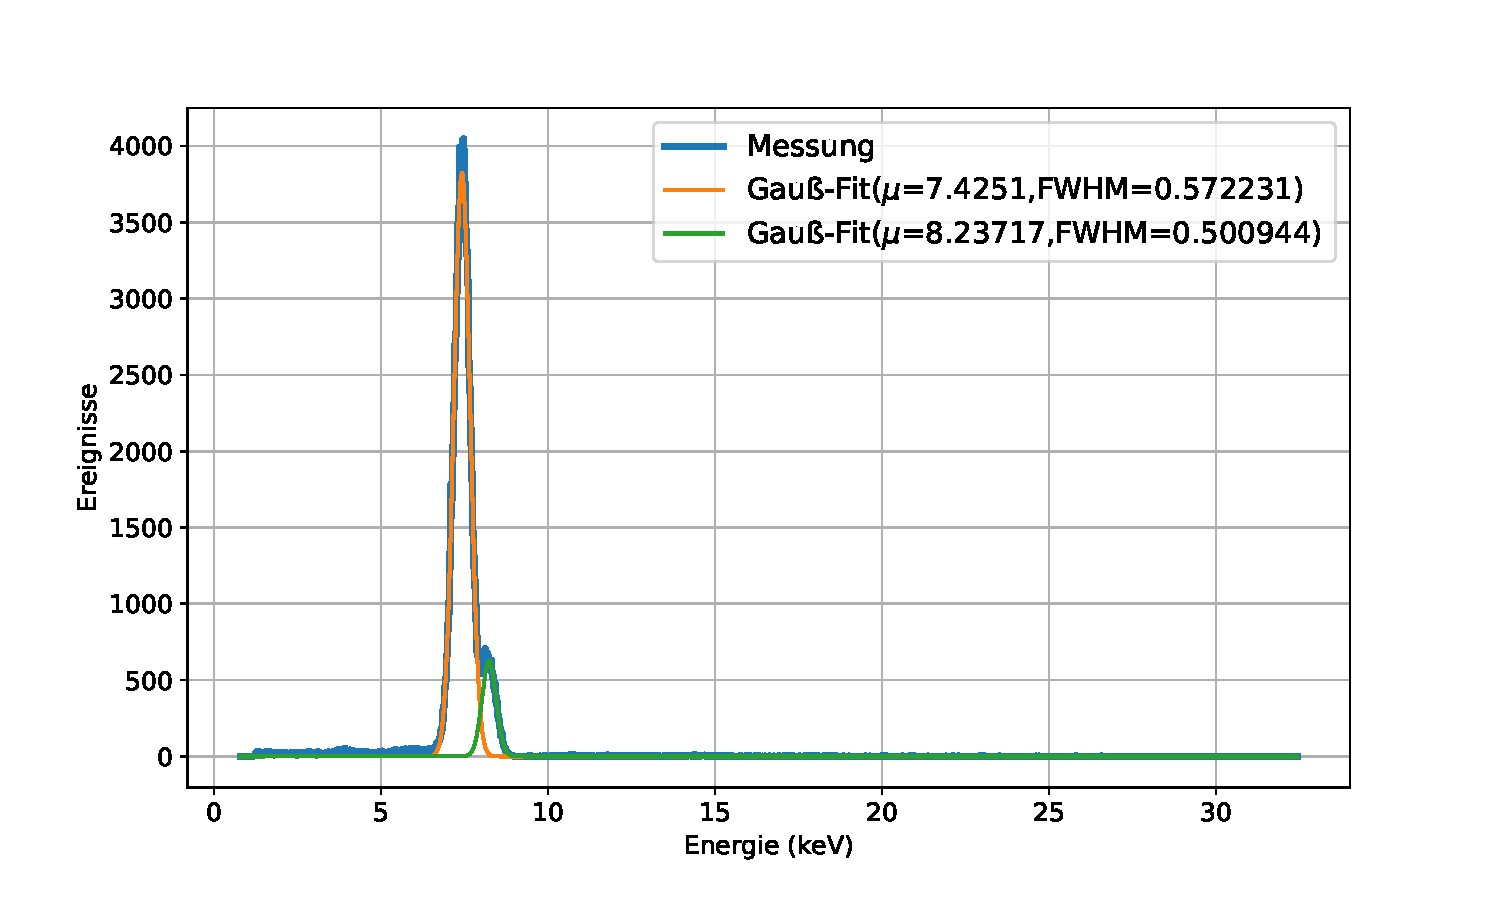
\includegraphics[width=\textwidth]{images/10-X.pdf}
		\centering
		\caption{Röntgenfluoreszenzspektrum der Probe 10.}
	\end{figure}

	\begin{figure}[H]
		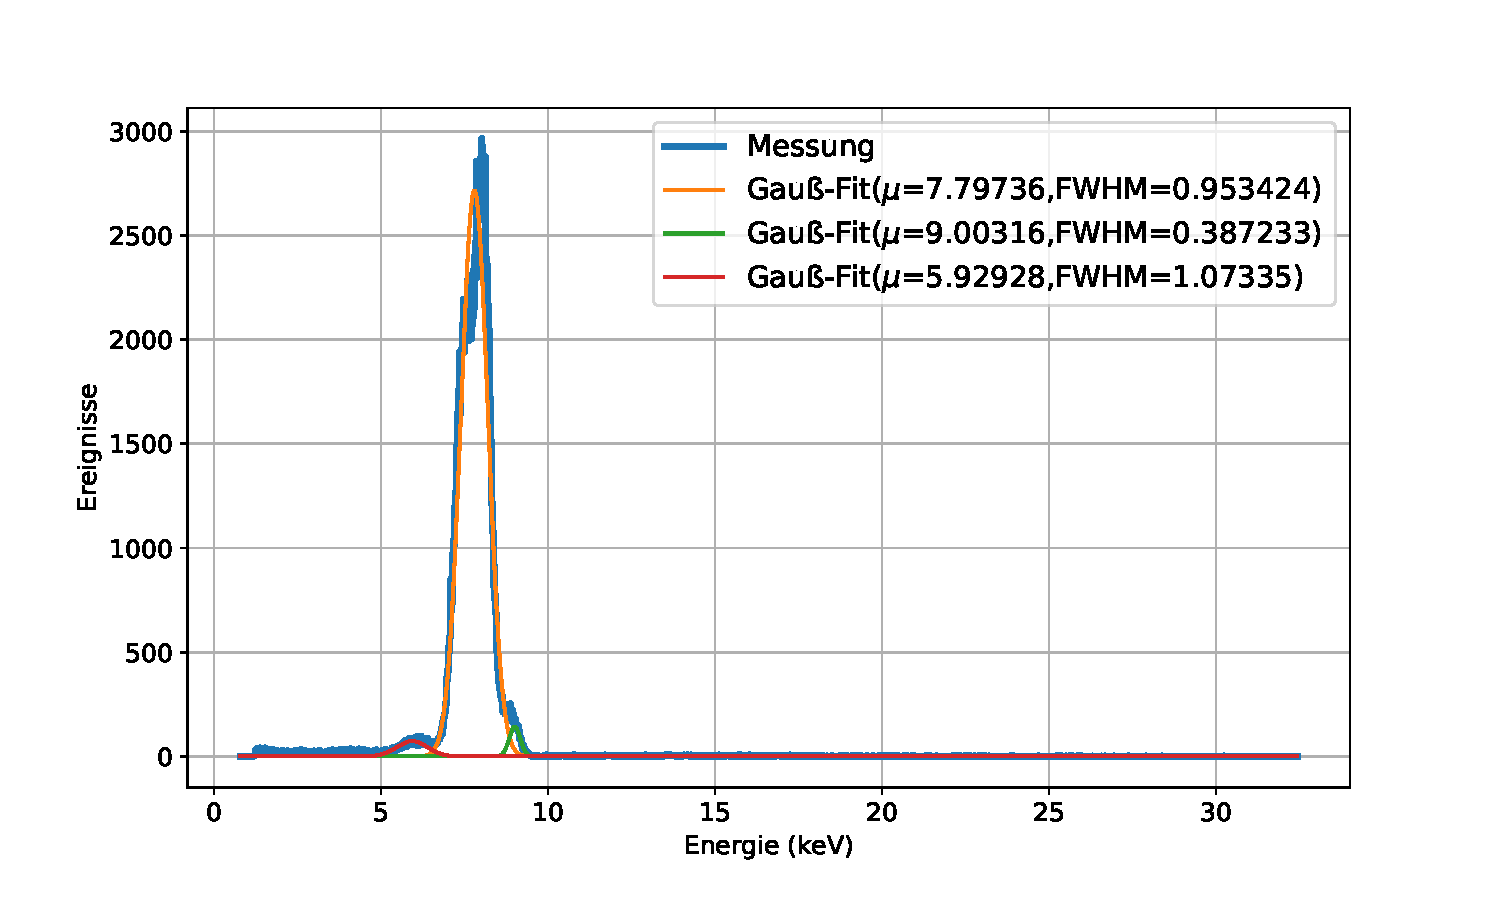
\includegraphics[width=\textwidth]{images/11-X.pdf}
		\centering
		\caption{Röntgenfluoreszenzspektrum der Probe 11.}
	\end{figure}

	\begin{figure}[H]
		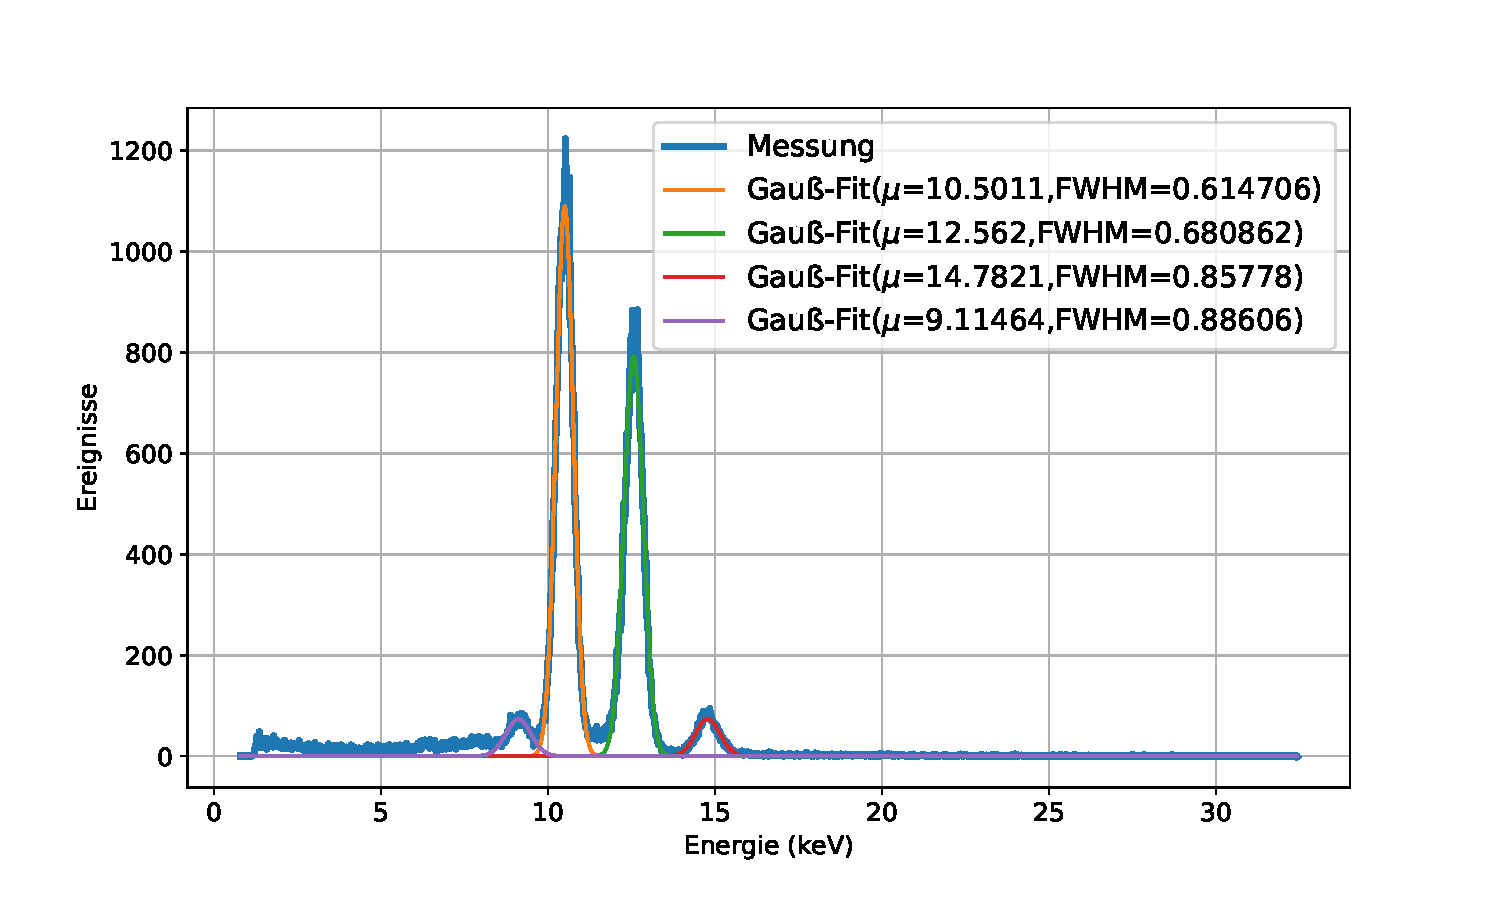
\includegraphics[width=\textwidth]{images/12-X.pdf}
		\centering
		\caption{Röntgenfluoreszenzspektrum der Probe 12.}
	\end{figure}

	\begin{figure}[H]
		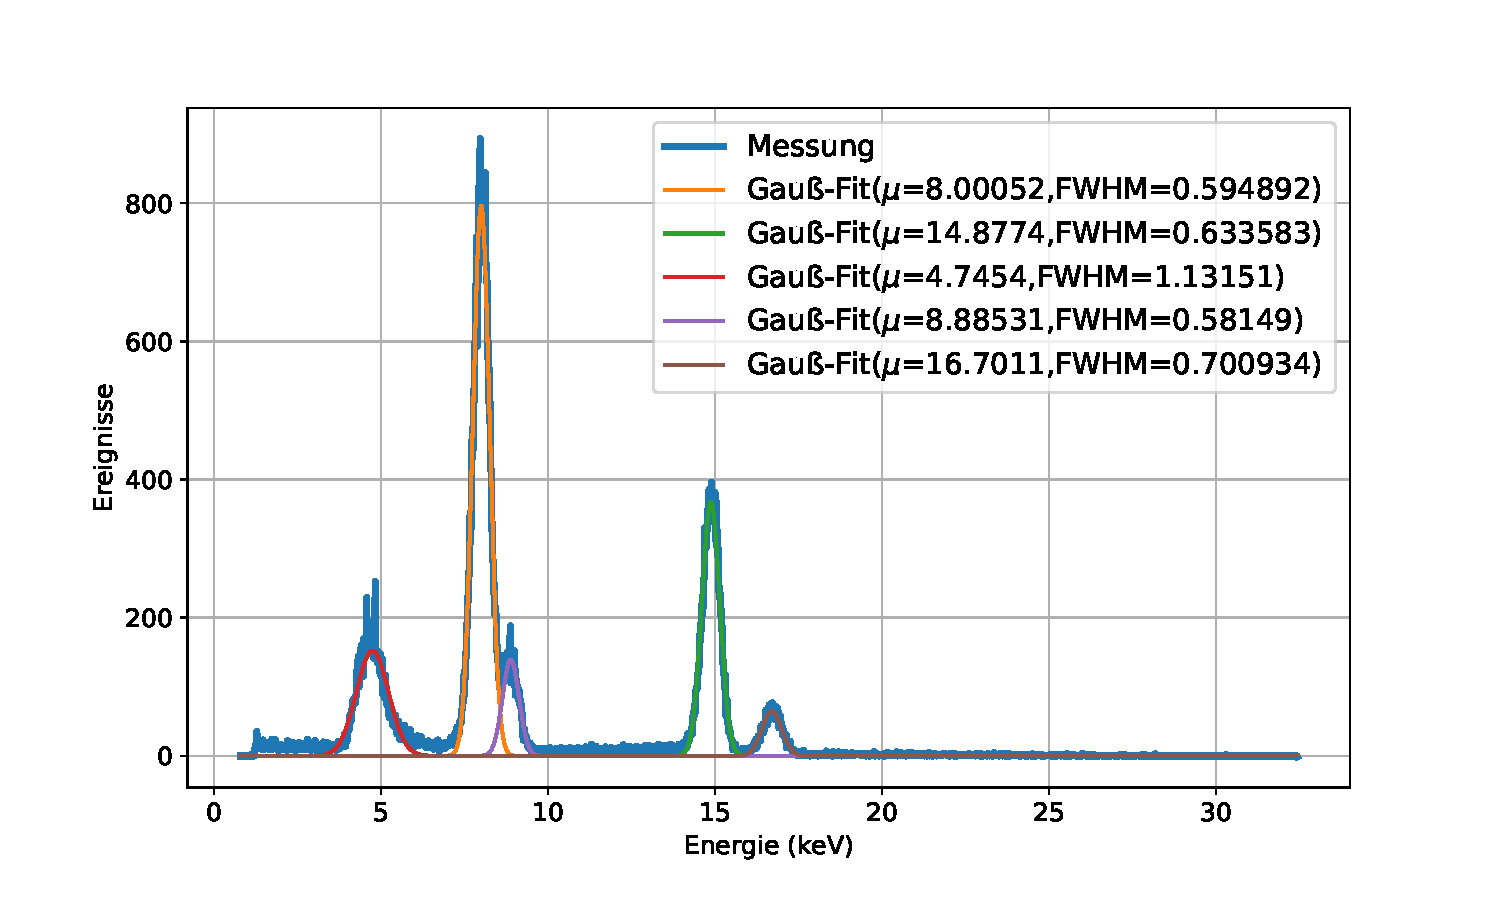
\includegraphics[width=\textwidth]{images/13-X.pdf}
		\centering
		\caption{Röntgenfluoreszenzspektrum der Probe 13.}
	\end{figure}

	\begin{figure}[H]
		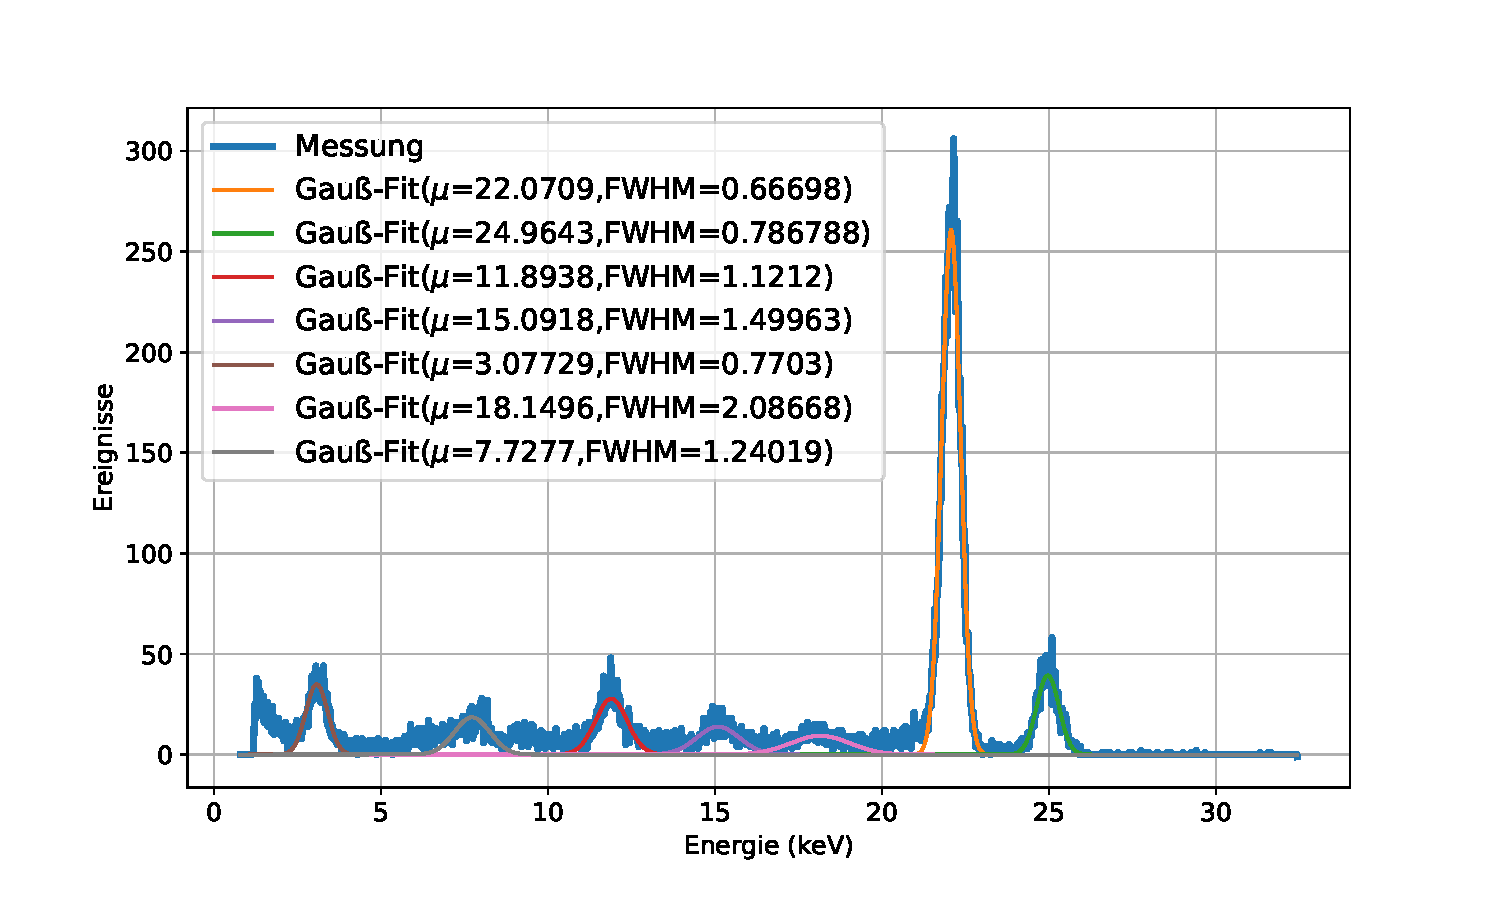
\includegraphics[width=\textwidth]{images/14-X.pdf}
		\centering
		\caption{Röntgenfluoreszenzspektrum der Probe 14.}
	\end{figure}

	\begin{figure}[H]
		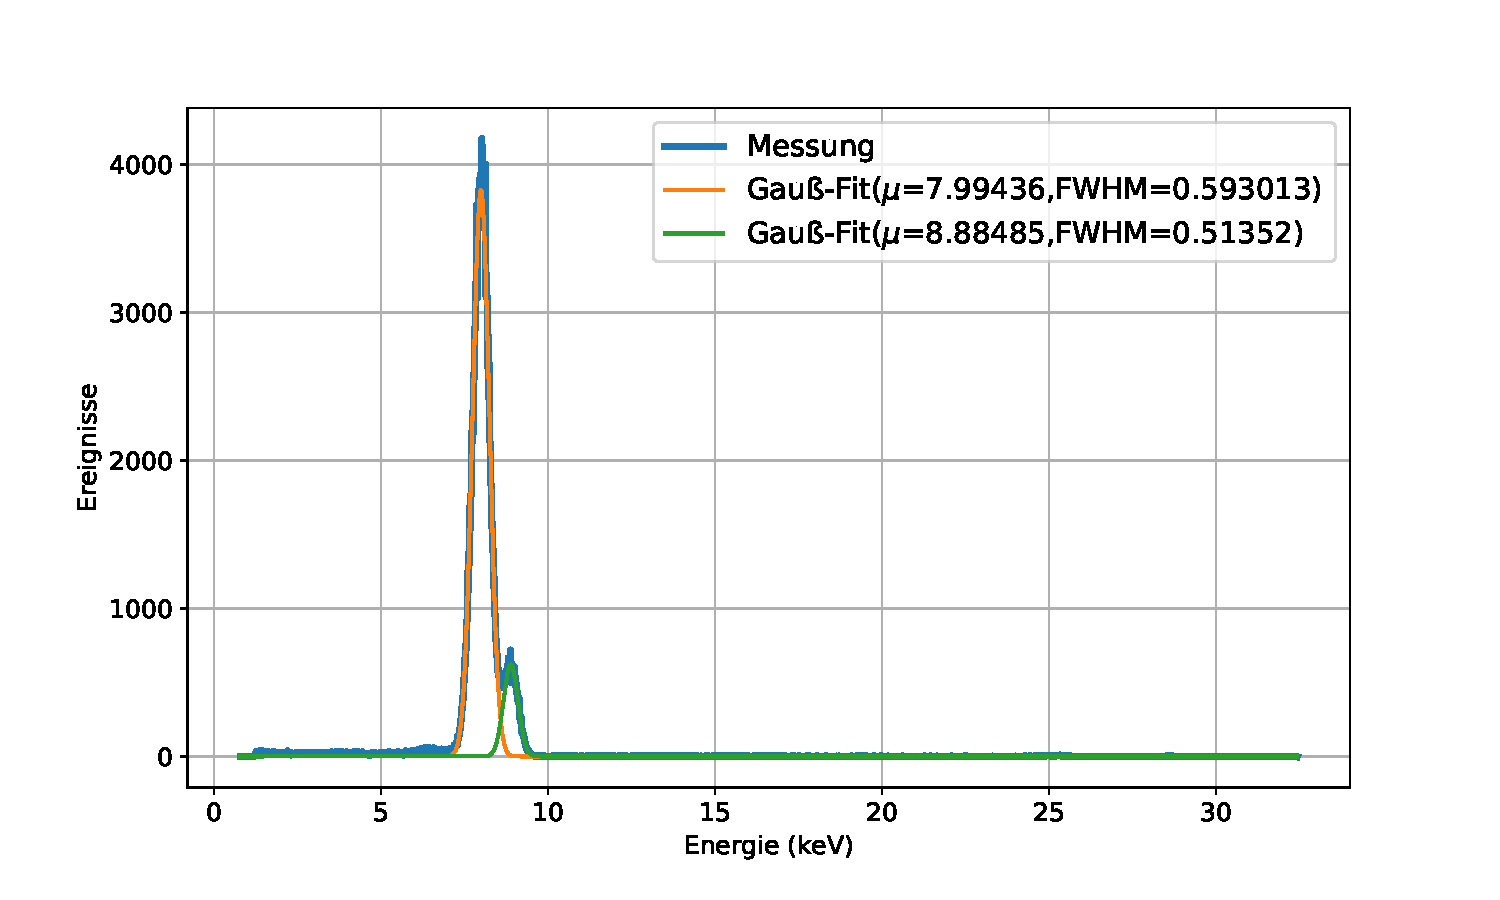
\includegraphics[width=\textwidth]{images/15-X.pdf}
		\centering
		\caption{Röntgenfluoreszenzspektrum der Probe 15.}
	\end{figure}

	\begin{figure}[H]
		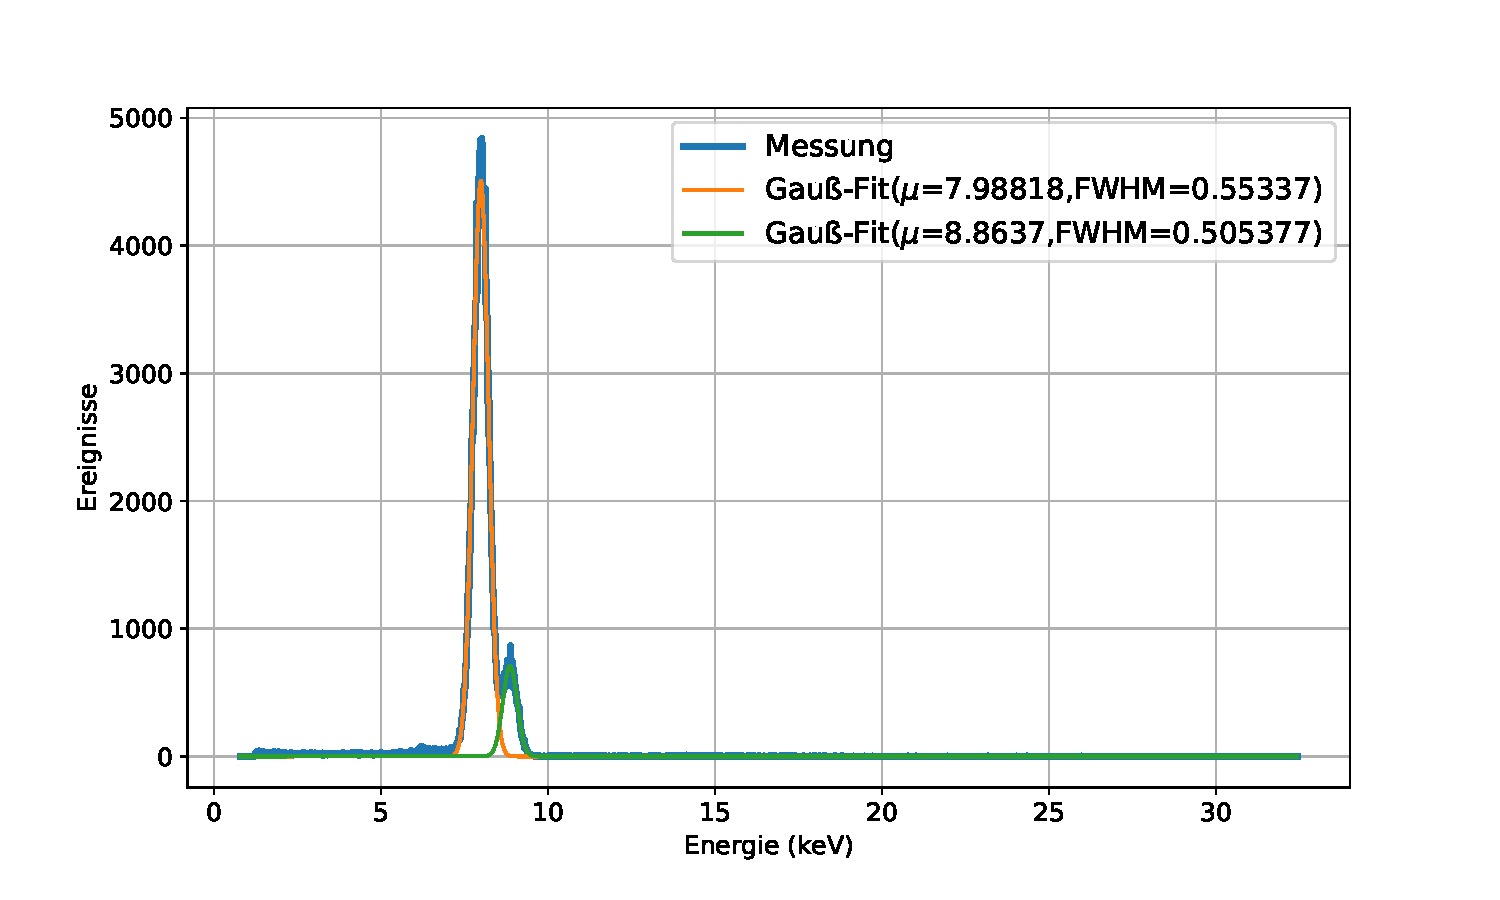
\includegraphics[width=\textwidth]{images/16-1-Cent.pdf}
		\centering
		\caption{Röntgenfluoreszenzspektrum der Probe 16.}
	\end{figure}

	\begin{figure}[H]
		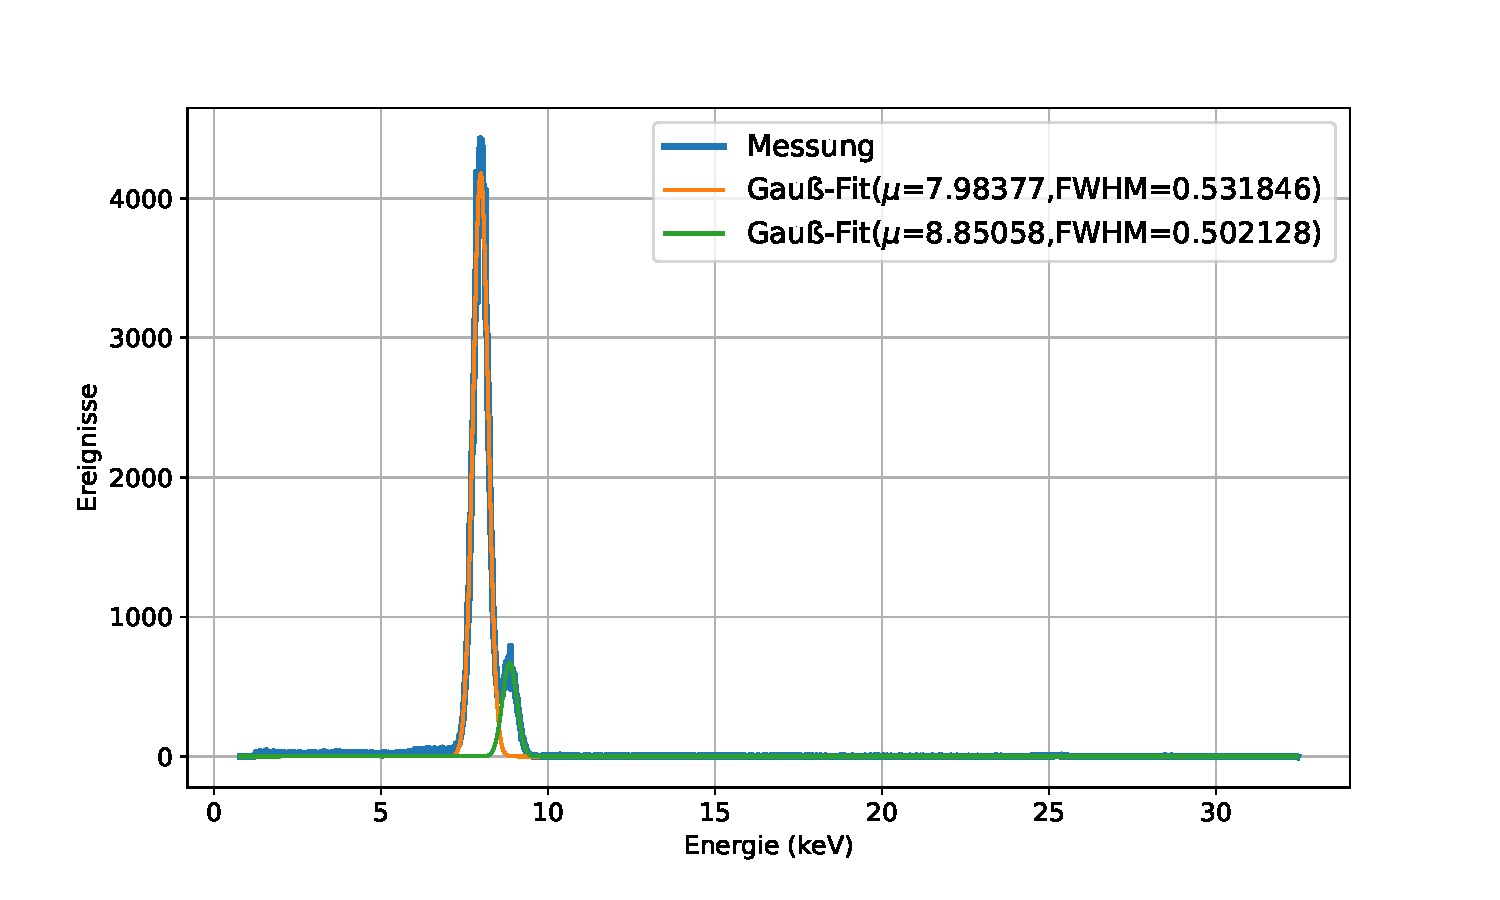
\includegraphics[width=\textwidth]{images/17-X.pdf}
		\centering
		\caption{Röntgenfluoreszenzspektrum der Probe 17.}
	\end{figure}

	\begin{figure}[H]
		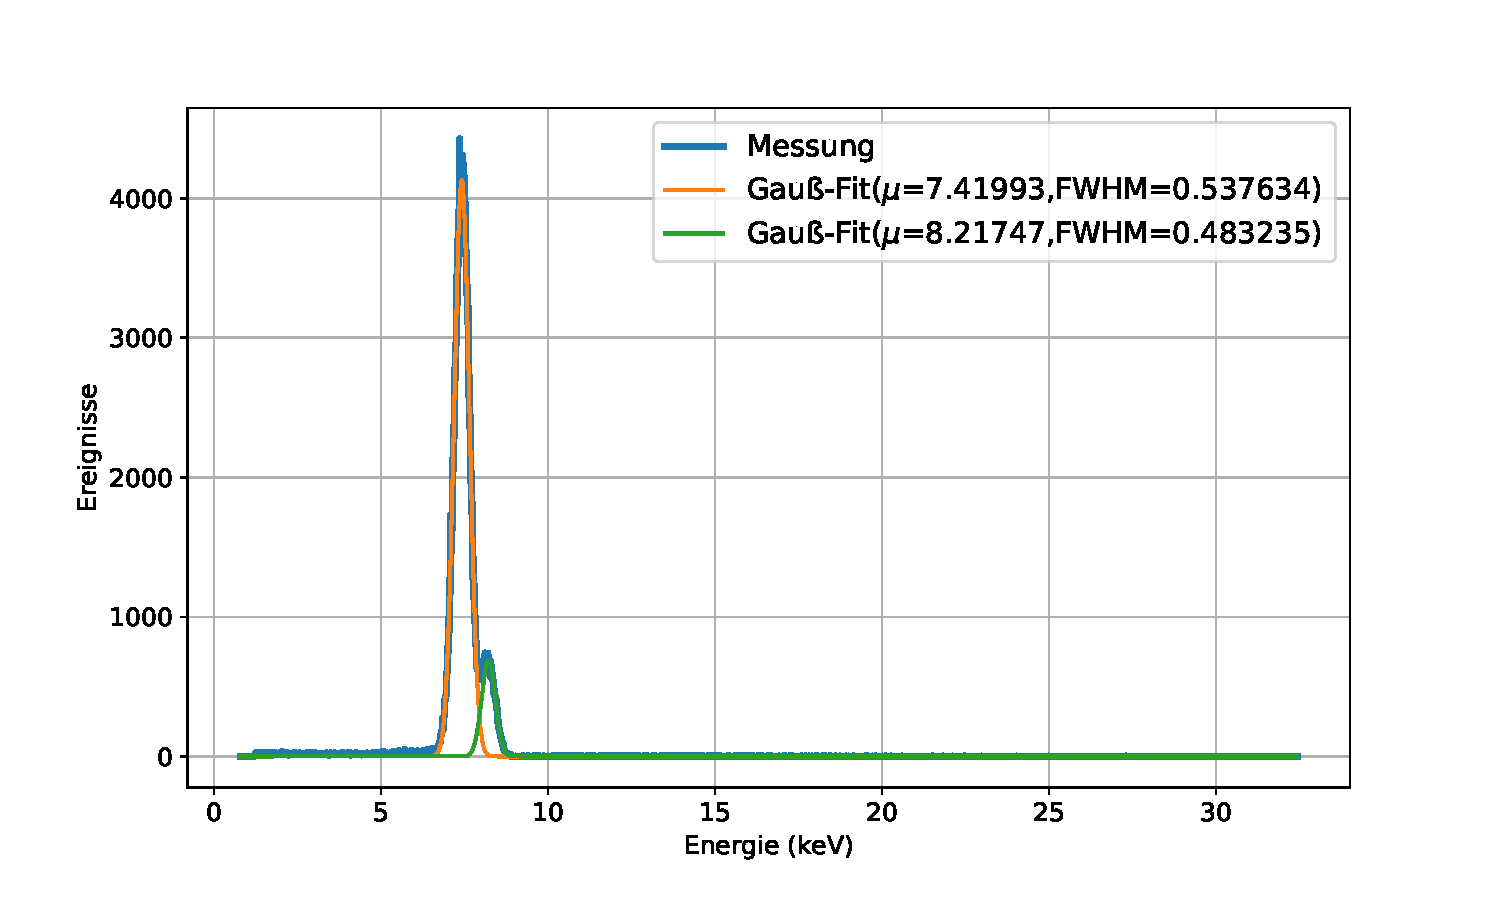
\includegraphics[width=\textwidth]{images/18-X.pdf}
		\centering
		\caption{Röntgenfluoreszenzspektrum der Probe 18.}
	\end{figure}

	\begin{figure}[H]
		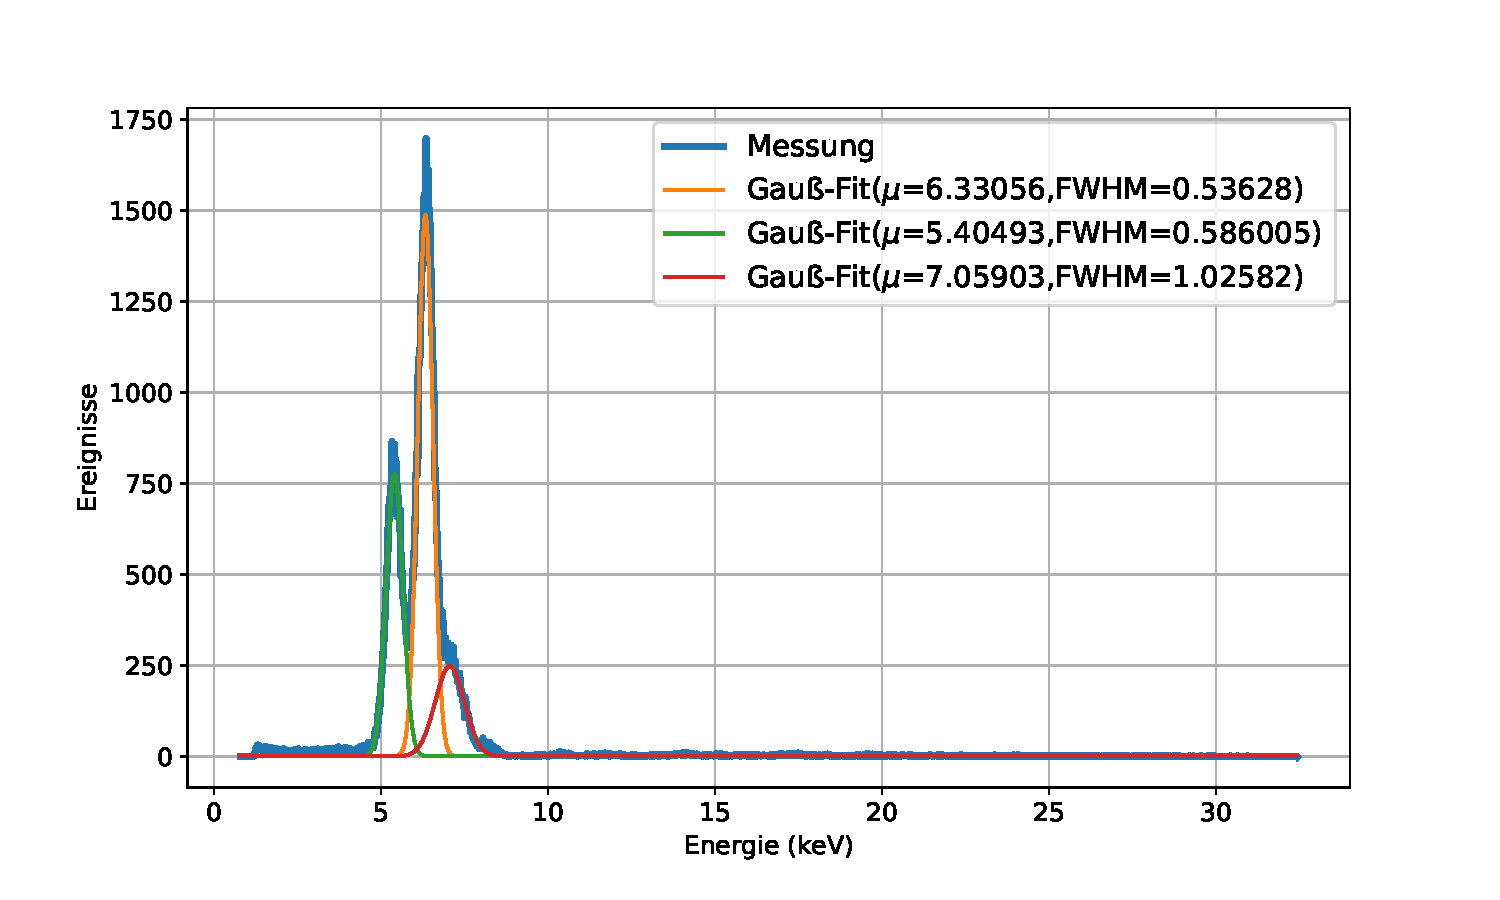
\includegraphics[width=\textwidth]{images/19-X.pdf}
		\centering
		\caption{Röntgenfluoreszenzspektrum der Probe 19.}
	\end{figure}

	\begin{figure}[H]
		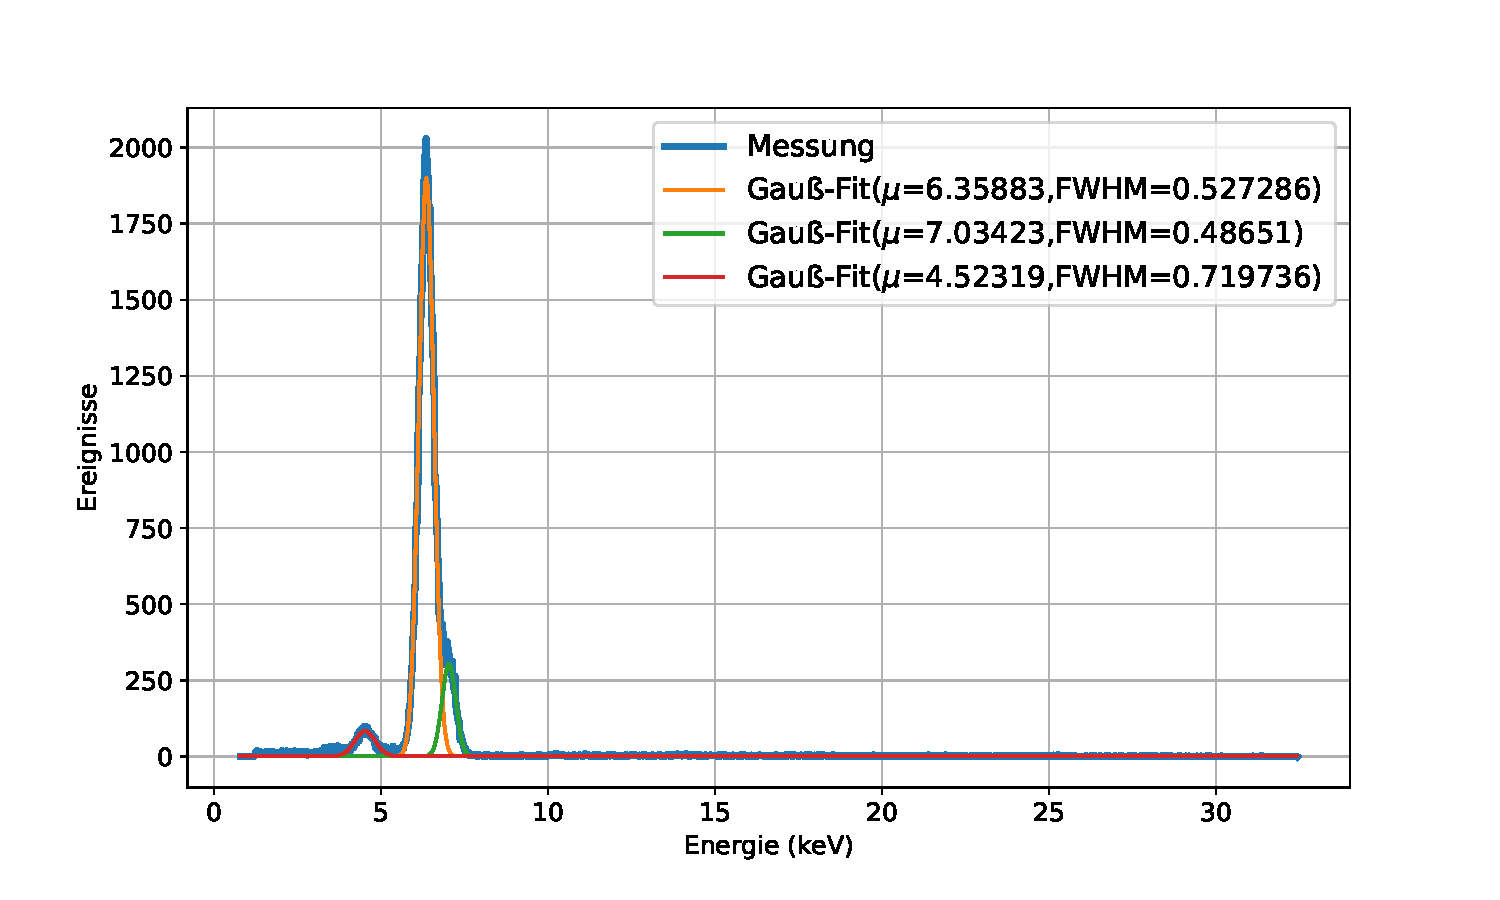
\includegraphics[width=\textwidth]{images/20-Kronkorken.pdf}
		\centering
		\caption{Röntgenfluoreszenzspektrum der Probe 20.}
	\end{figure}

\begin{figure}[H]
		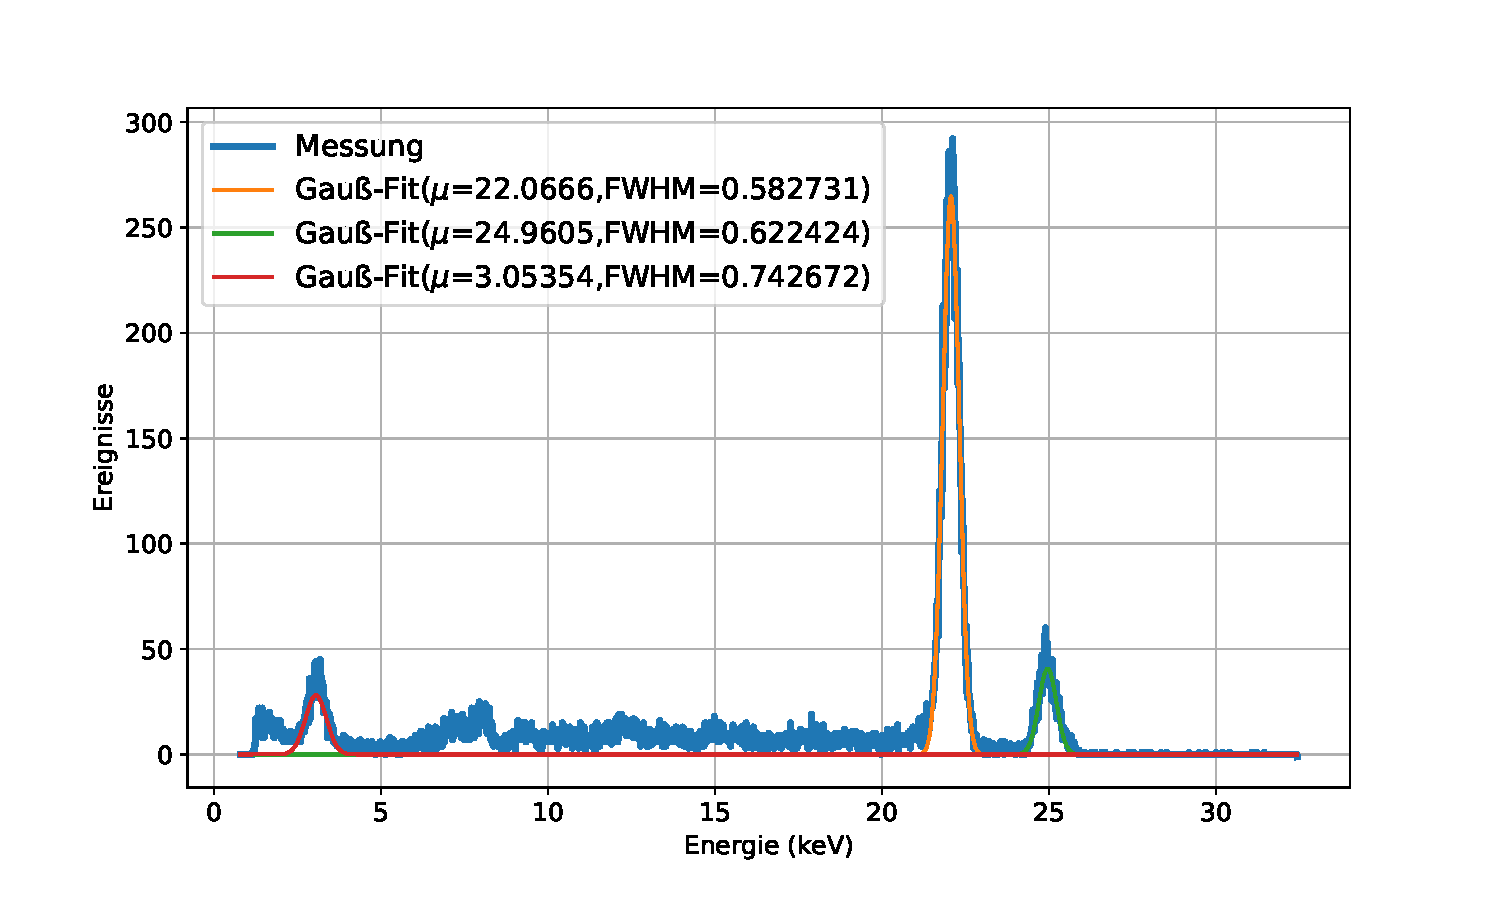
\includegraphics[width=\textwidth]{images/21-Ag.pdf}
		\centering
		\caption{Röntgenfluoreszenzspektrum der Probe 21.}
	\end{figure}

\end{document}
